\chapter{Sviluppo e implementazione}
\label{cha:sviluppo_implementazione}

\section{Tecnologie utilizzate}
\label{sec:tecnologie}

Le tecnologie utilizzate per l'implementazione di questo bot saranno descritte brevemente di seguito. 

\subsection{Node.js}

\begin{wrapfigure}{r}{0.33\textwidth}
\centering

\includegraphics[width=2.5cm]{nodejs-logo.png}
\caption{Logo NodeJS}
\end{wrapfigure}

\textit{Node.js} è un runtime JavaScript guidato da eventi asincroni ed è progettato per creare applicazioni di rete scalabili. Alcuni dei principali vantaggi di Nodejs sono le ottime performance, un processo di sviluppo facilitato e un'ottima scalabilità. Inoltre, utilizzandolo si ha accesso al più grande ecosistema di librerie open source al mondo: \textit{Node Package Manager} (NPM).

\subsection{telegraf.js}

\begin{wrapfigure}{r}{0.33\textwidth}
\centering

\includegraphics[width=2.5cm]{telegraf-logo.png}
\caption{Logo telegraf.js}
\end{wrapfigure}

Telegram per creare i bot mette a disposizione della API HTTPS. Lo sviluppatore può scegliere se utilizzarle come sono fornite oppure avvalersi di una delle tante librerie esistenti per i principali linguaggi di programmazione. Esse sono ormai il metodo suggerito, poiché semplificano molto lo sviluppo e offrono la possibilità di aggiungere funzionalità extra. Per Node.js esistono varie librerie, io ho scelto di utilizzare \textit{telegraf.js} perché ritengo sia la più completa ed è molto supportata dalla comunità. Essa è anche estensibile attraverso ulteriori librerie che danno la possibilità di introdurre altre feature.

\subsection{MongoDB}

\begin{wrapfigure}{r}{0.33\textwidth}
\centering

\includegraphics[width=3cm]{mongodb-logo.png}
\caption{Logo MongoDB}
\end{wrapfigure}

\textit{MongoDB} è un DBMS non relazionale, orientato ai documenti. Classificato come un database di tipo NoSQL, MongoDB si allontana dalla struttura tradizionale basata su tabelle dei database relazionali in favore di documenti in stile JSON con schema dinamico (MongoDB chiama il formato BSON), rendendo l'integrazione di dati di alcuni tipi di applicazioni più facile e veloce \cite{Mongodb}. Le principali caratteristiche sono che la replicazione di un database (\textit{Replica Set}) può avvenire in modo molto semplice, e che garantisce la scalabilità automatica, ossia la possibilità di distribuire (Sharding) le collezioni in cluster di nodi, in modo da supportare grandi quantità di dati senza influire pesantemente sulle performance.

\subsection{Redis}

\begin{wrapfigure}{r}{0.33\textwidth}
\centering

\includegraphics[width=3cm]{redis-logo.png}
\caption{Logo Redis}
\end{wrapfigure}

\textit{Redis}, acronimo di Remote Dictionary Server, è un archivio dati veloce, open source, in memoria e di tipo chiave-valore. Esso può essere utilizzato come database, sistema di caching o come broker di messaggi. Redis offre tempi di risposta inferiori al millisecondo ed è per questo una scelta popolare per caching, gestione della sessione, giochi, classifiche, analisi dei dati in tempo reale, geospazialità, ride-hailing, chat/messaggistica, streaming multimediale. \cite{Redis}

\pagebreak

\section{Implementazione}
\label{sec:implementazione}

Per l'implementazione di questo bot ho scelto di utilizzare \textit{NodeJs} utilizzando \textit{Typescript} come linguaggio di programmazione. \textit{Typescript} mi ha permesso di utilizzare la programmazione ad oggetti e di tipizzare le risposte ottenute dalle API, rendendo il codice molto più strutturato e solido.  Durante lo sviluppo mi sono avvalso di alcune librerie presenti su NPM tra cui \textit{telegraf.js} per l'implementazione delle chiamate alle API di Telegram, \textit{Axios} per poter chiamare in modo agevole le API dei servizi esterni descritti in precedenza e \textit{mongoose} per potermi interfacciare con il database MongoDB.

Per gestire le sessioni ho utilizzato un estensione della libreria telegraf.js che permette di salvare e gestire la sessione degli utenti nel database MongoDB, questo ha semplificato la gestione dei flussi più complessi che richiedono all'utente di inserire più informazioni. 

\subsection{Architettura}
\label{sec:architettura}

L'architettura del bot Telegram è rappresentata in figura \ref{fig:architettura_bot}.

\begin{figure}[h]
\centering
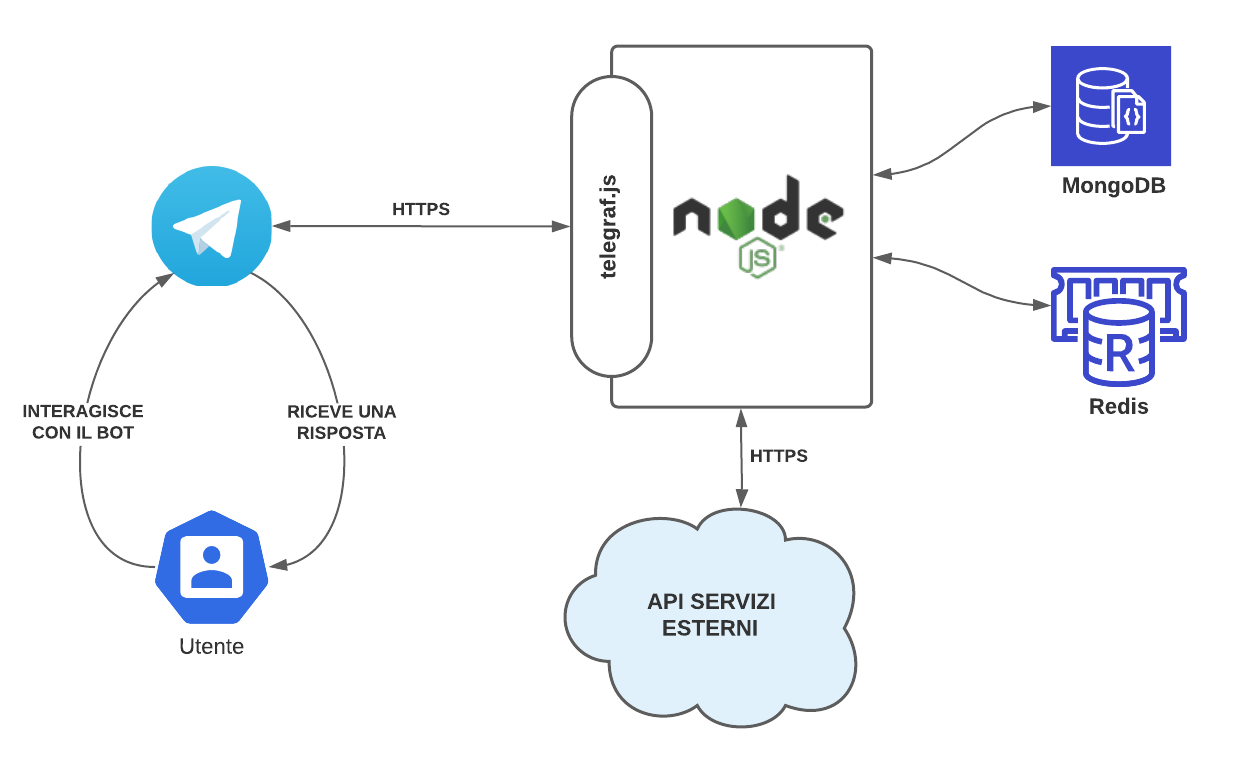
\includegraphics[width=0.9\textwidth]{architettura-bot.png}
\caption{Architettura del bot}
\label{fig:architettura_bot}
\end{figure}

Come si può osservare dalla figura, quando un utente invia una richiesta (messaggio, comando, posizione, ...) dall'applicazione Telegram, le informazioni vengono processate dai server di quest'ultima e sono rese disponibili attraverso le Bot API. La libreria \textit{telegraf.js} si occupa, quindi, dell'interazione con queste API rendendole disponibili al backend \textit{Nodejs}. Il backend si occupa di gestire le informazioni ricevute e restituisce all'utente una risposta adeguata. Per fare ciò potrà avvalersi dei servizi esterni e dei database. Il database MongoDB è utilizzato sia per mantenere le sessioni e le preferenze degli utenti che per memorizzare gli orari degli autobus mentre Redis è utilizzato come sistema di caching. Maggiori dettagli sullo scopo e l'utilizzo dei database sono adeguatamente forniti nel paragrafo \ref{sec:problemi}.

\pagebreak

\noindent Di seguito un esempio concreto: 
\begin{enumerate} 
\item l'utente invia al bot, attraverso un comando, una richiesta di orario per la fermata Piazza Dante; 
\item la richiesta viene processata dai server di Telegram, e resa disponibile attraverso una Bot API;
\item il backend di \textit{Node.js}, attraverso l'interfaccia \textit{telegraf.js}, riceve l'informazione;
\item il backend contatta il database per estrarre gli orari e l'API esterna per l'informazione in tempo reale;
\item una volta raccolte tutte le informazioni, \textit{Node.js} formatterà un messaggio di risposta; 
\item questo verrà inviato, attraverso le Bot API, a Telegram; 
\item l'utente riceverà la risposta sul proprio dispositivo. 
\end{enumerate}

\noindent In figura \ref{fig:bpmn_autobus_flow} è rappresentato, attraverso l'utilizzo di un \textit{Business Process Modeling Notation} (BPMN), il processo di richiesta e visualizzazione degli orari di una fermata autobus urbana. Il diagramma è stato semplificato in modo da raffigurare solo il flusso principale e tralasciando la gestione dei casi limite.

\begin{figure}[h]
\centering
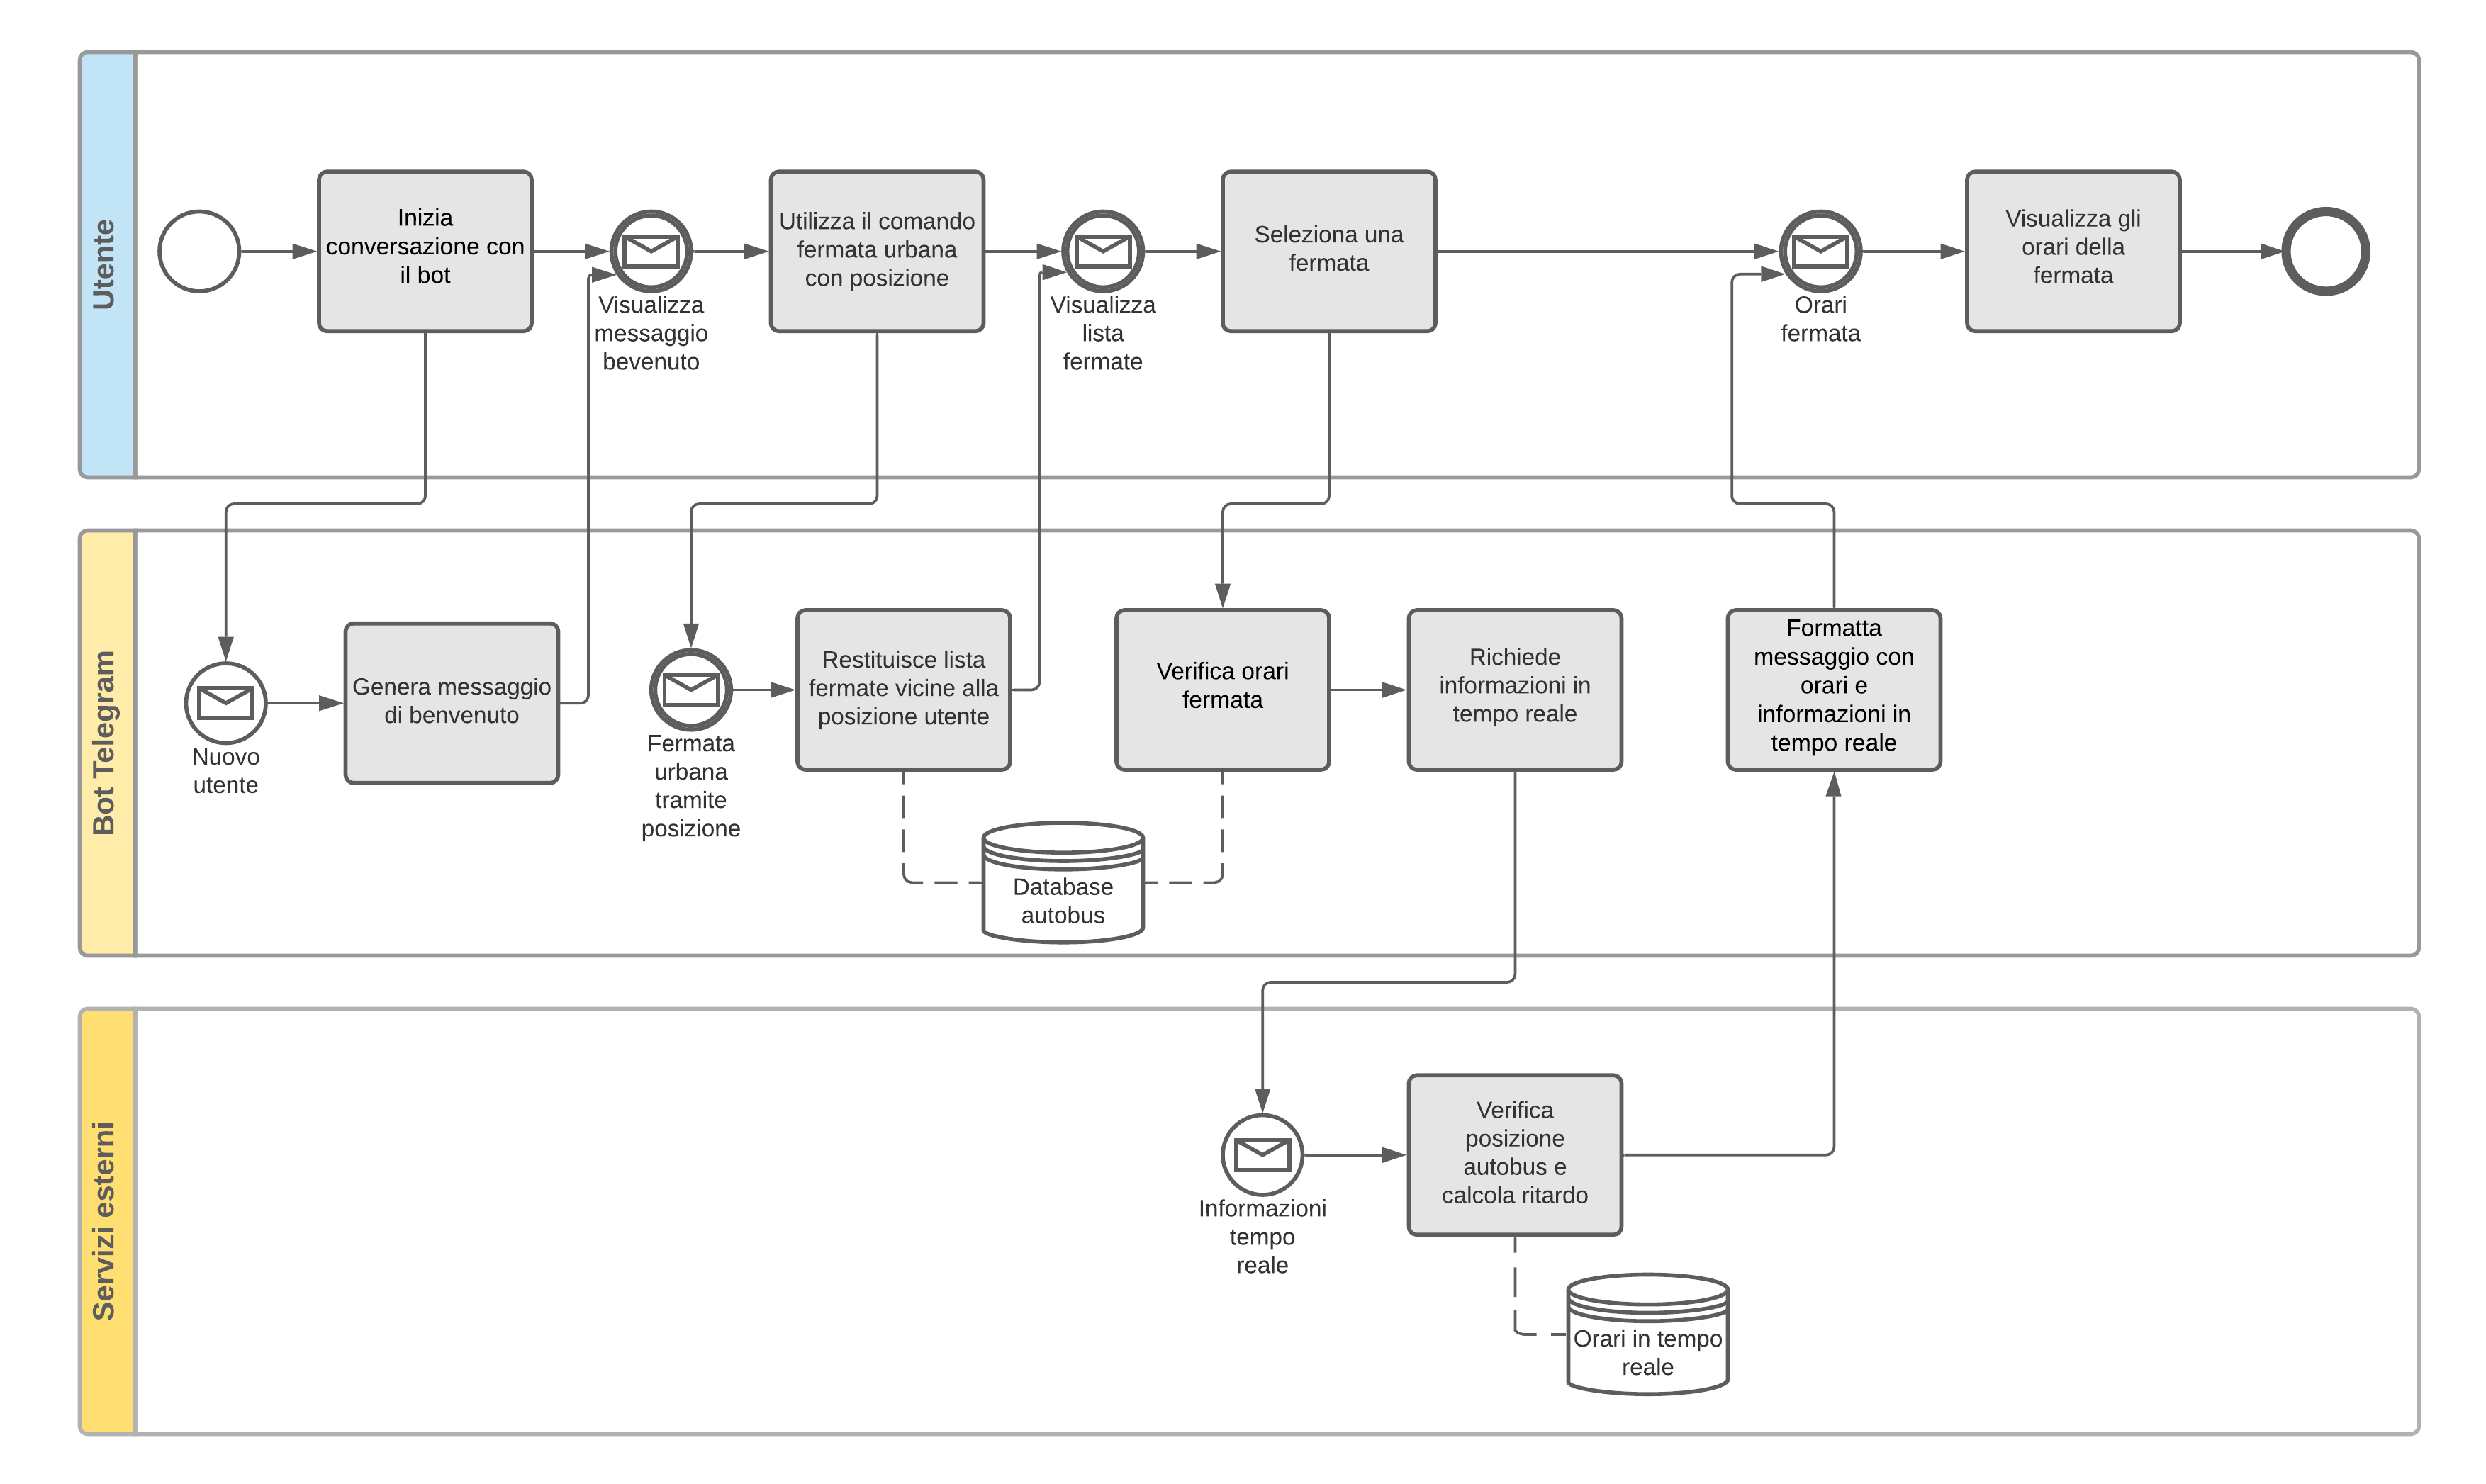
\includegraphics[width=\textwidth]{bot-bpmn-autobus-flow.png}
\caption{BPMN flusso richiesta orari fermata autobus}
\label{fig:bpmn_autobus_flow}
\end{figure}

\newpage
\newpage

\subsection{Continuous deployment e ambiente di produzione}
\label{sec:produzione}

Per l'hosting dell'applicativo \textit{Node.JS} ho deciso di utilizzare una VPS Ubuntu fornita dal provider tedesco \textit{Hetzner}. Sulla macchina virtuale ho poi installato un process manager, \textit{PM2}. Esso permette di semplificare alcuni compiti da amministratore di sistema, come riavviare l'applicativo in caso di crash, aggiornare il sistema senza avere momenti di inattività, mantenere e monitorare i log e implementa anche un sistema di load-balancing. Dato che il codice del bot è salvato su una repository Github, ho potuto utilizzare le \textit{Github Actions} per implementare un sistema di \textit{continuous deployment}. Ad ogni push sulla master branch viene attivato il flusso di pubblicazione che transpila il codice da Typescript a Javascript e copia quest'ultimo nella VPS ubuntu utilizzando il protocollo SSH. Grazie alla funzionalità di PM2, che permette di riavviare il programma in caso di cambiamenti nel codice, dopo pochi secondi la nuova versione è pubblicata e disponibile agli utenti. Il database Redis è installato e presente all'interno della VPS mentre il database MongoDB è esterno in un hosting \textit{Google Cloud} dedicato.

\begin{figure}[h]
\centering
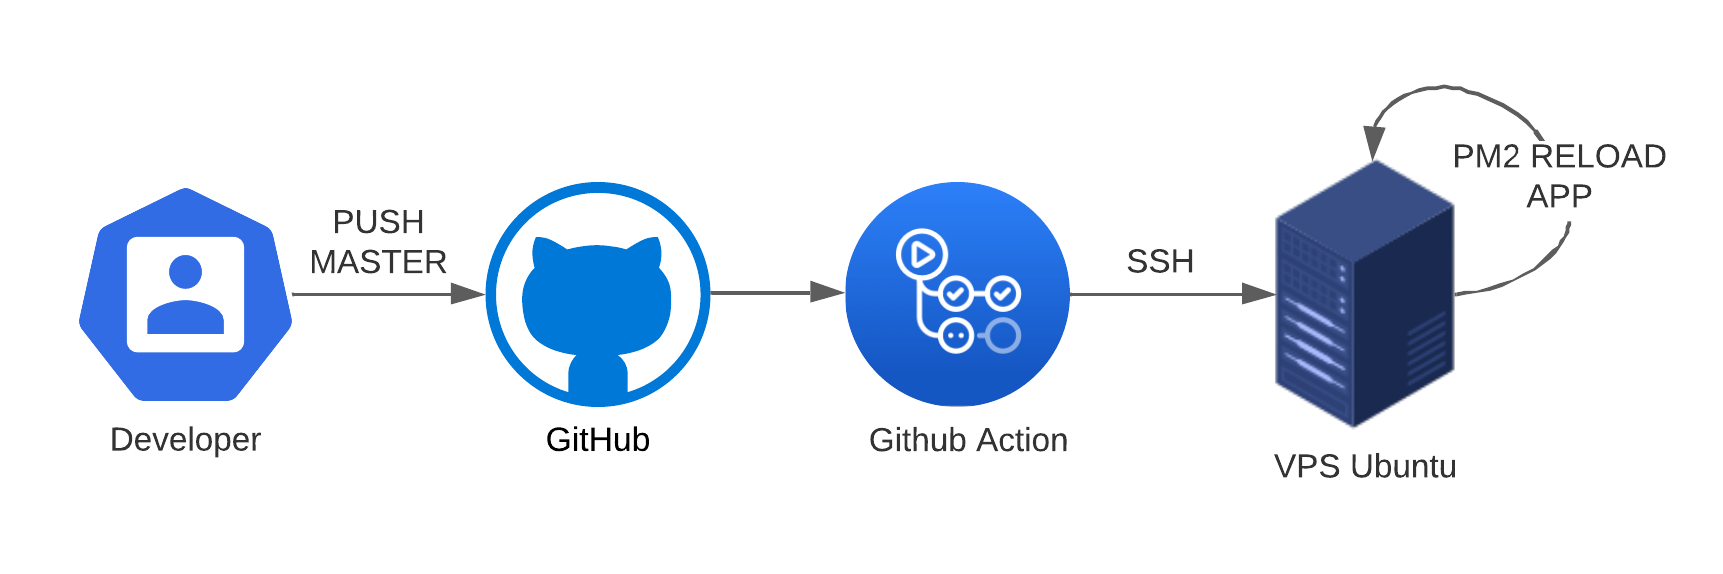
\includegraphics[width=0.90\textwidth]{continuous-deployment.png}
\caption{Flusso di distribuzione continua}
\label{fig:continuous_deployment}
\end{figure}

\section{Analisi dei principali problemi}
\label{sec:problemi}

Durante lo sviluppo di questo Bot ho incontrato alcuni problemi. La difficoltà maggiore riguarda la gestione delle API esterne che, a volte, non risultano disponibili. Per mitigare questo problema ho, in primo luogo, inserito dei messaggi di errore che informavano l'utente della presenza di un problema riscontrato non dipendente dal Bot, ma dai servizi esterni. 
In particolare, le API che presentano maggiormente questo problema sono quelle che restituiscono le informazioni in tempo reale degli autobus. In un primo momento, queste API venivano utilizzate anche per conoscere gli orari, ma data la frequente assenza di questi dati, ho deciso di aggiungere al database \textit{MongoDB} una copia di tutte le informazioni sulle fermate e sulle linee. Questo permette di chiamare l'API solo per i dati in tempo reale, permettendo comunque all'utente di ricevere gli orari con l'avviso della temporanea mancanza dei ritardi e della posizione. 
Dopo l'introduzione di questa soluzione, ho notato che le risposte all'utente, vista la necessità del doppio passaggio, richiedevano dei tempi di caricamento maggiori. Per ovviare a questo problema, ho introdotto un sistema di \textit{caching} del database \textit{MongoDB} utilizzando \textit{Redis} e ho implementato anche un sistema di \textit{caching} per le risposte ottenute dall'API esterne. Ciò ha permesso di migliorare l'esperienza dell'utente, riducendo sensibilmente i tempi di risposta. 

\newpage

\section{Funzionamento ed interfaccia utente}
\label{sec:funzionamento}

La sezione seguente è dedicata all'analisi, attraverso la presentazione dell'interfaccia utente, del funzionamento generale e delle caratteristiche del bot. La descrizione è accompagnata da alcune schermate tratte dall'applicazione mobile di Telegram in modo da rendere più chiaro di cosa si sta parlando.

\subsection{Menu iniziale}

\begin{wrapfigure}{r}{0.45\textwidth}
\centering
\frame{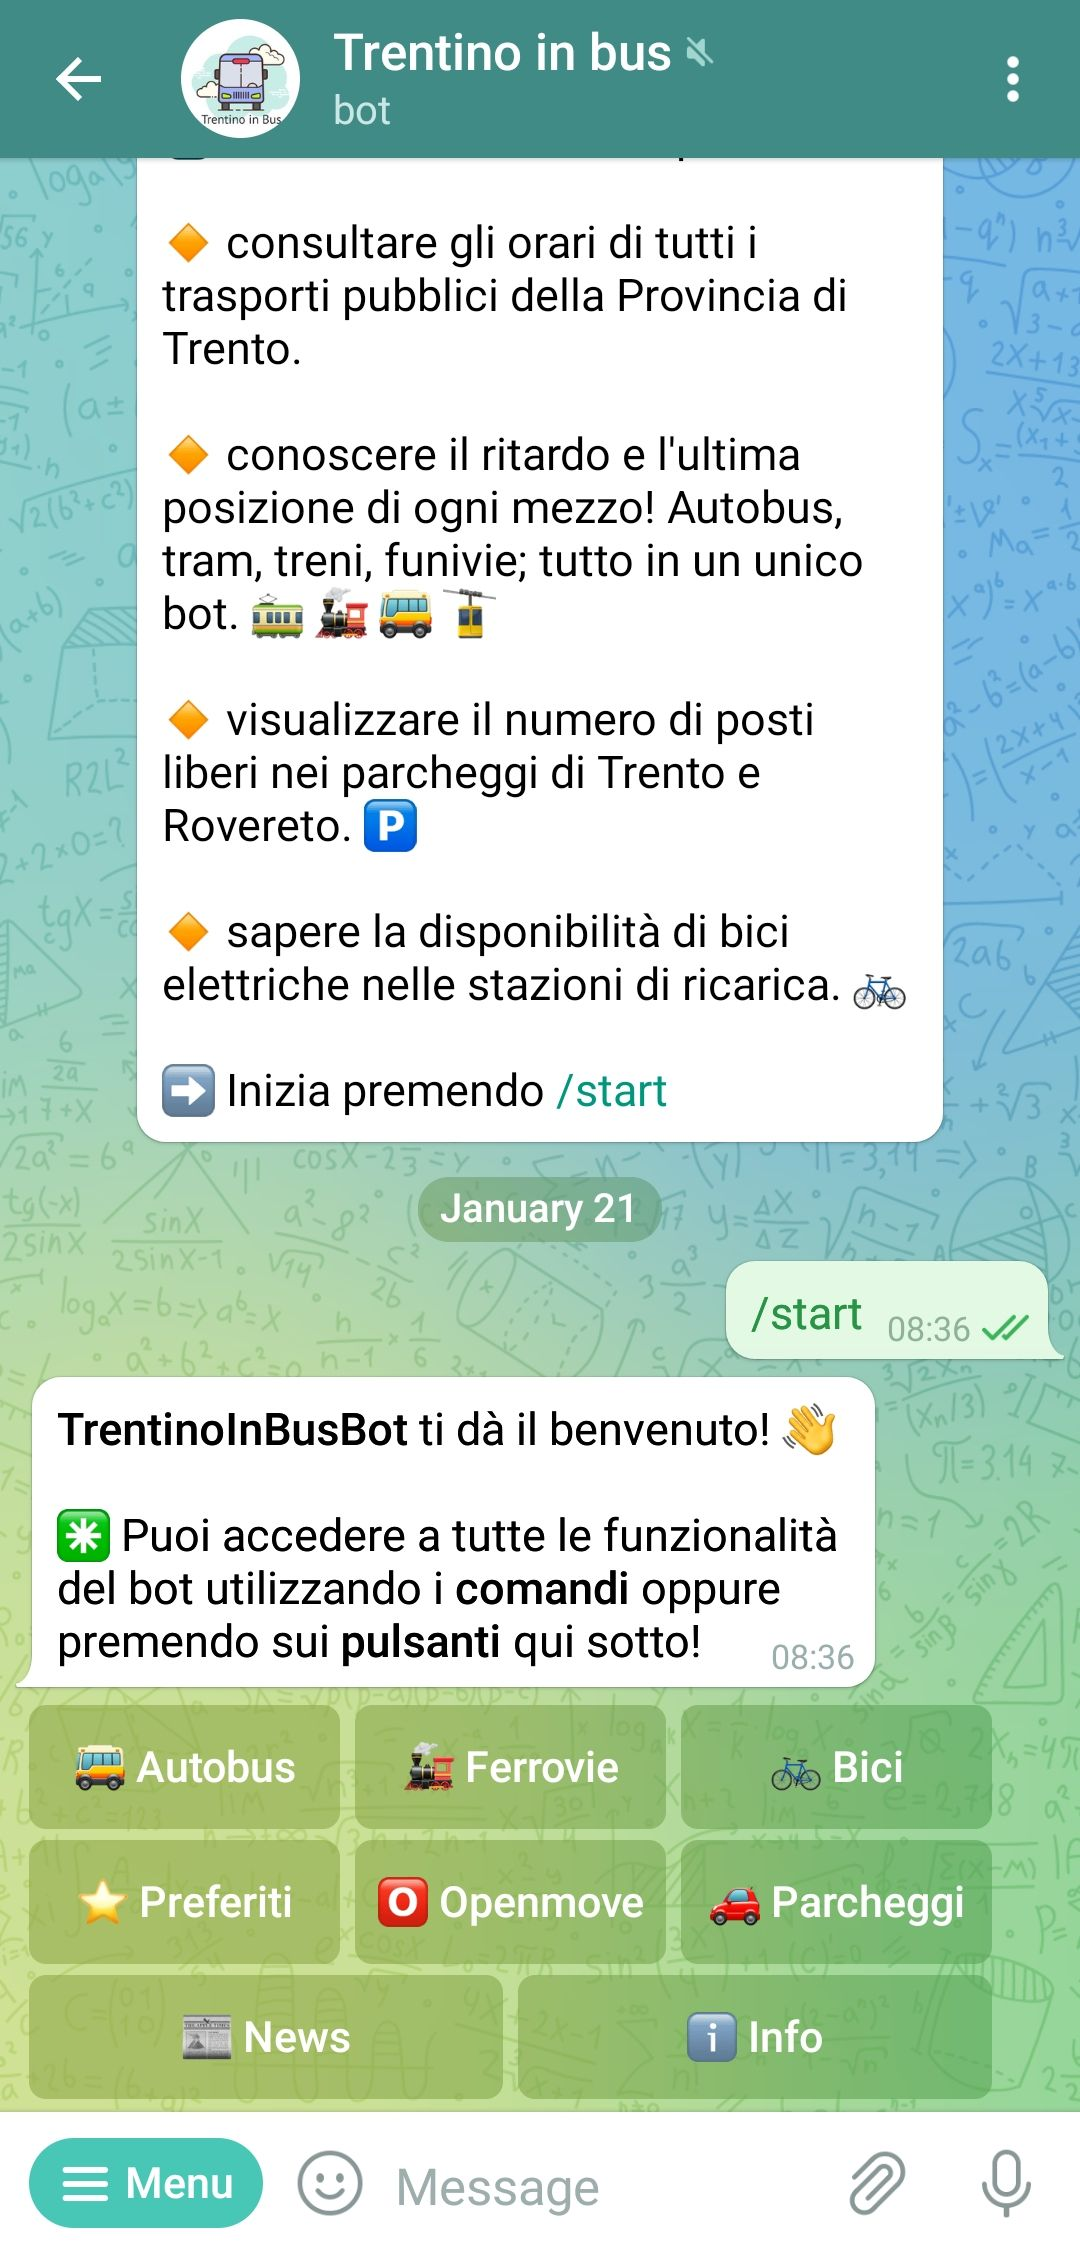
\includegraphics[scale=0.14]{bot-menu-iniziale.jpg}}
\caption{Menu iniziale}
\label{fig:bot-menu-iniziale}
\end{wrapfigure}

Una volta aperta la chat privata con il bot Telegram, \textit{@TrentinoInBusBot}, ci si trova davanti ad un messaggio di benvenuto che descrive brevemente le funzionalità del bot. Per iniziare è necessario inviare il comando \textit{/start}. L'utente riceverà a questo punto un messaggio con una \textit{tastiera inline}. Tramite quest'ultima, come si può notare nella figura \ref{fig:bot-menu-iniziale}, si è voluto creare un menu iniziale, che raggruppa in categorie le funzionalità principali, e da la possibilità di navigare ed utilizzare il bot in maniera semplice.

Come si vedrà anche successivamente, ogni messaggio inviato dal bot avrà sempre una \textit{tastiera inline} allegata che permette di ritornare al menu principale o di compiere diverse azioni a seconda della funzionalità che stiamo utilizzando. L'utilizzo di queste tastiere permette al bot di essere molto più simile ad un applicazione mobile tradizionale, di guidare l'utente e di essere intuitivo anche per utenti al primo utilizzo. Per rendere l'interfaccia più accattivante e accessibile sono state inserite delle \textit{emoji}.

In alternativa al menu principale, il bot mette a disposizione anche dei comandi scorciatoia che permettono di accedere alle funzionalità più velocemente. Ad esempio, un utente invece che premere sul pulsante \textit{Bici}, visibile in figura \ref{fig:bot-menu-iniziale}, potrebbe semplicemente utilizzare il comando \textit{/bici} e otterrebbe lo stesso risultato.

\subsection{Funzionalità autobus}

\begin{figure}[htb]
    \centering 
\begin{subfigure}{0.20\textwidth}
\frame{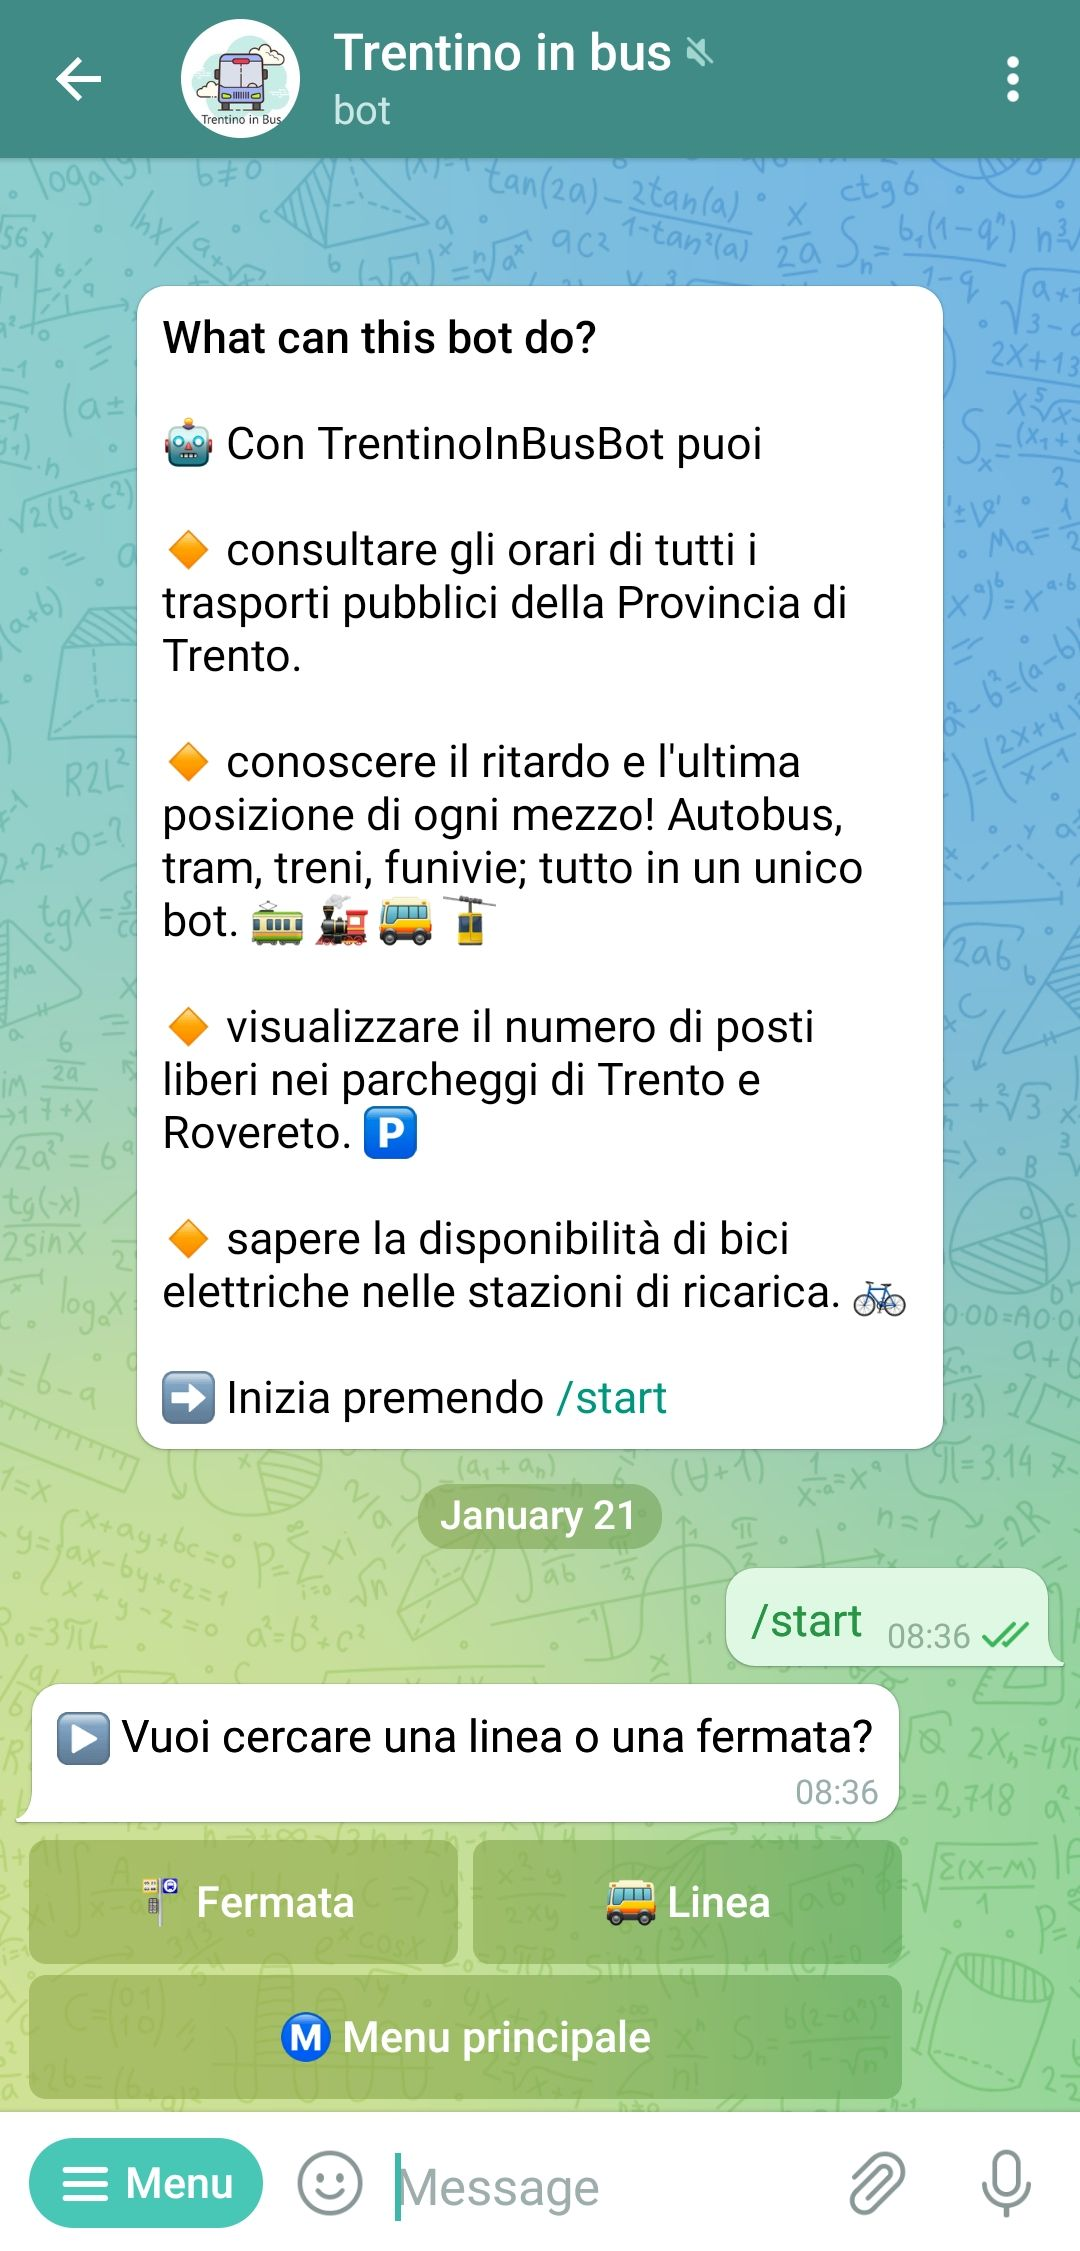
\includegraphics[width=\linewidth]{bot-selezione-autobus.jpg}}
\caption{Selezione ricerca}
\label{fig:bot-selezione-autobus}
\end{subfigure}\hfil
\begin{subfigure}{0.20\textwidth}
\frame{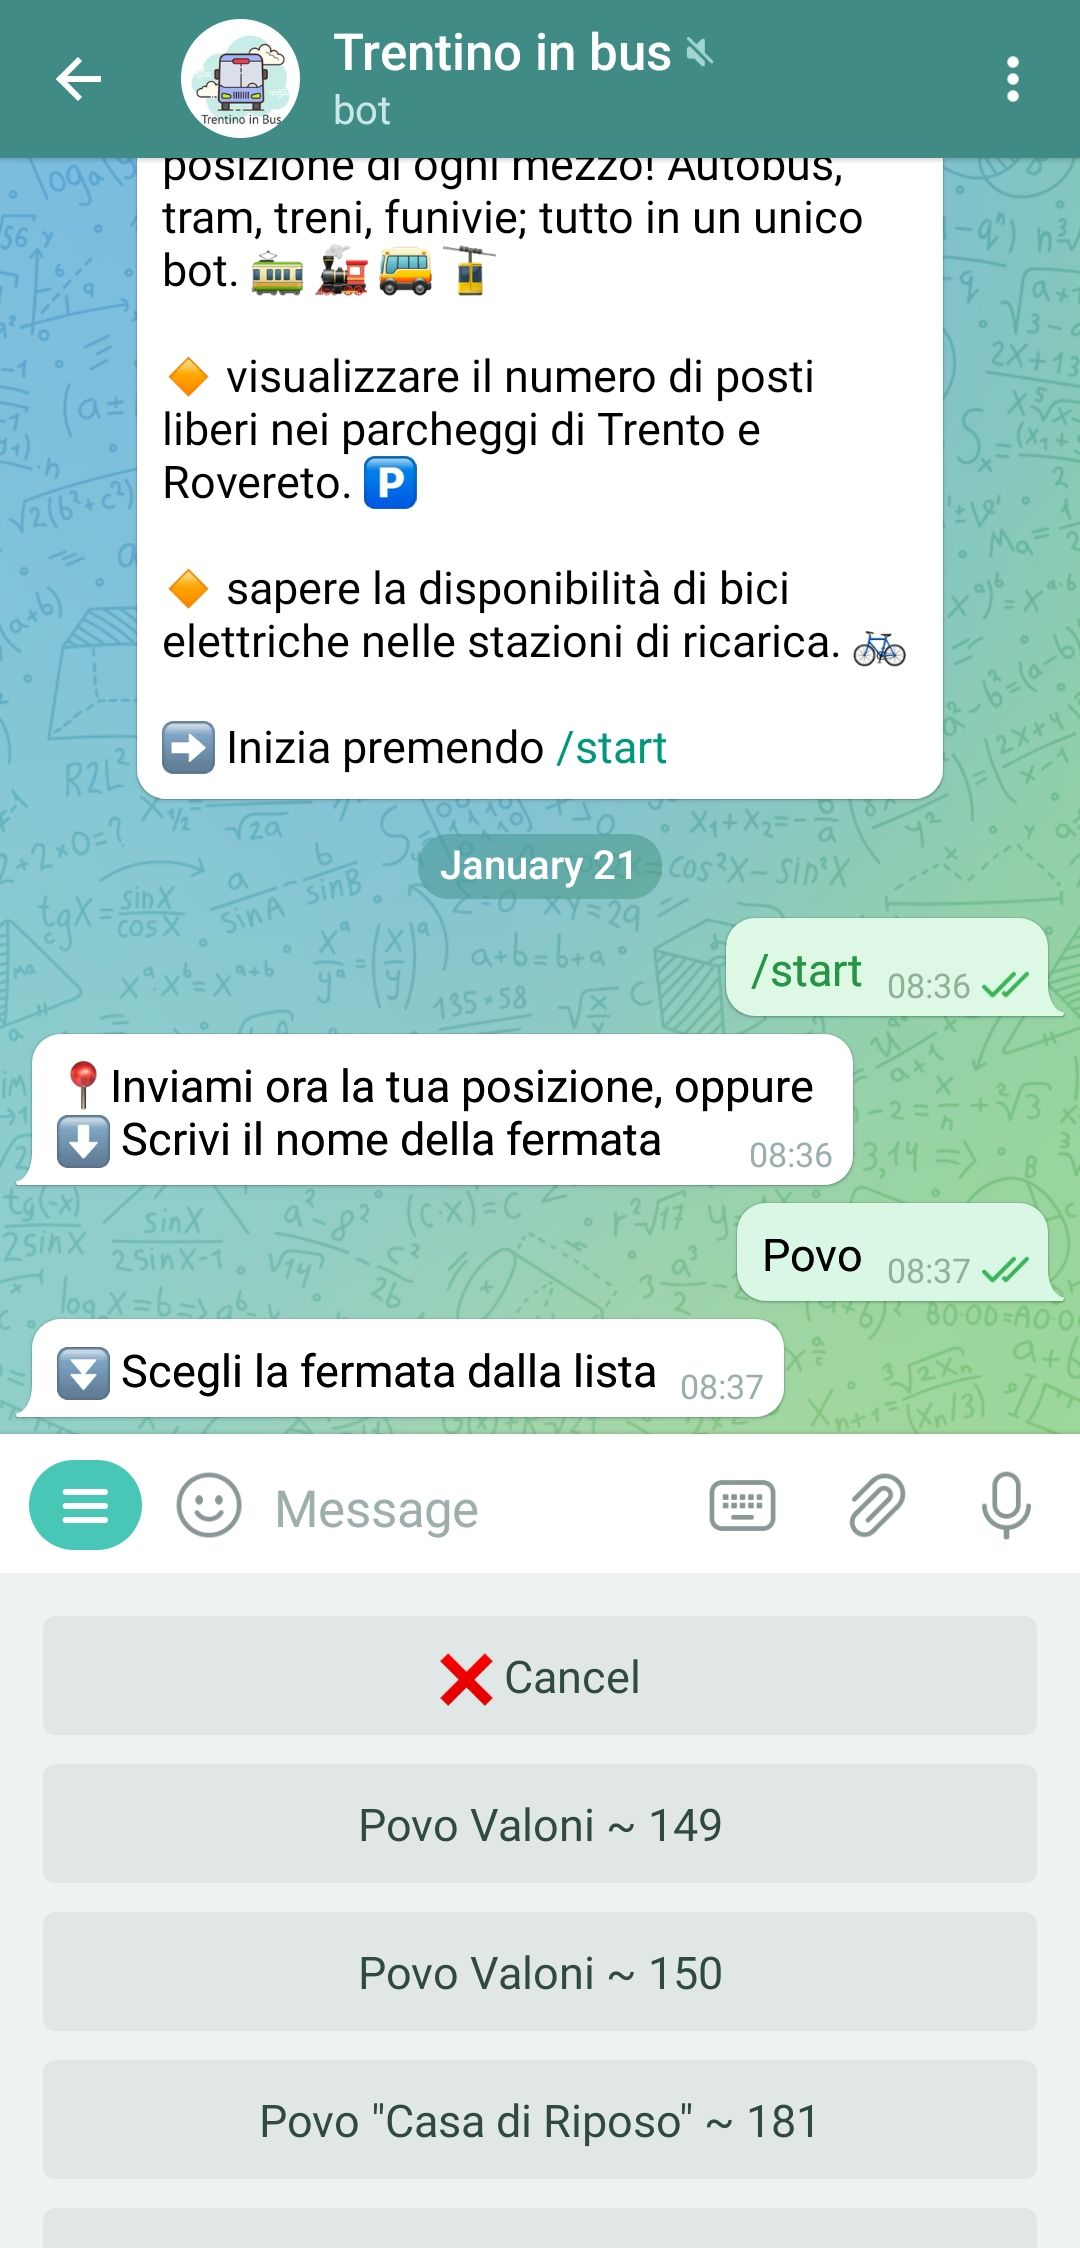
\includegraphics[width=\linewidth]{bot-selezione-fermata.jpg}}
\caption{Ricerca fermata}
\label{fig:bot-selezione-fermata}
\end{subfigure}\hfil 
\begin{subfigure}{0.20\textwidth}
\frame{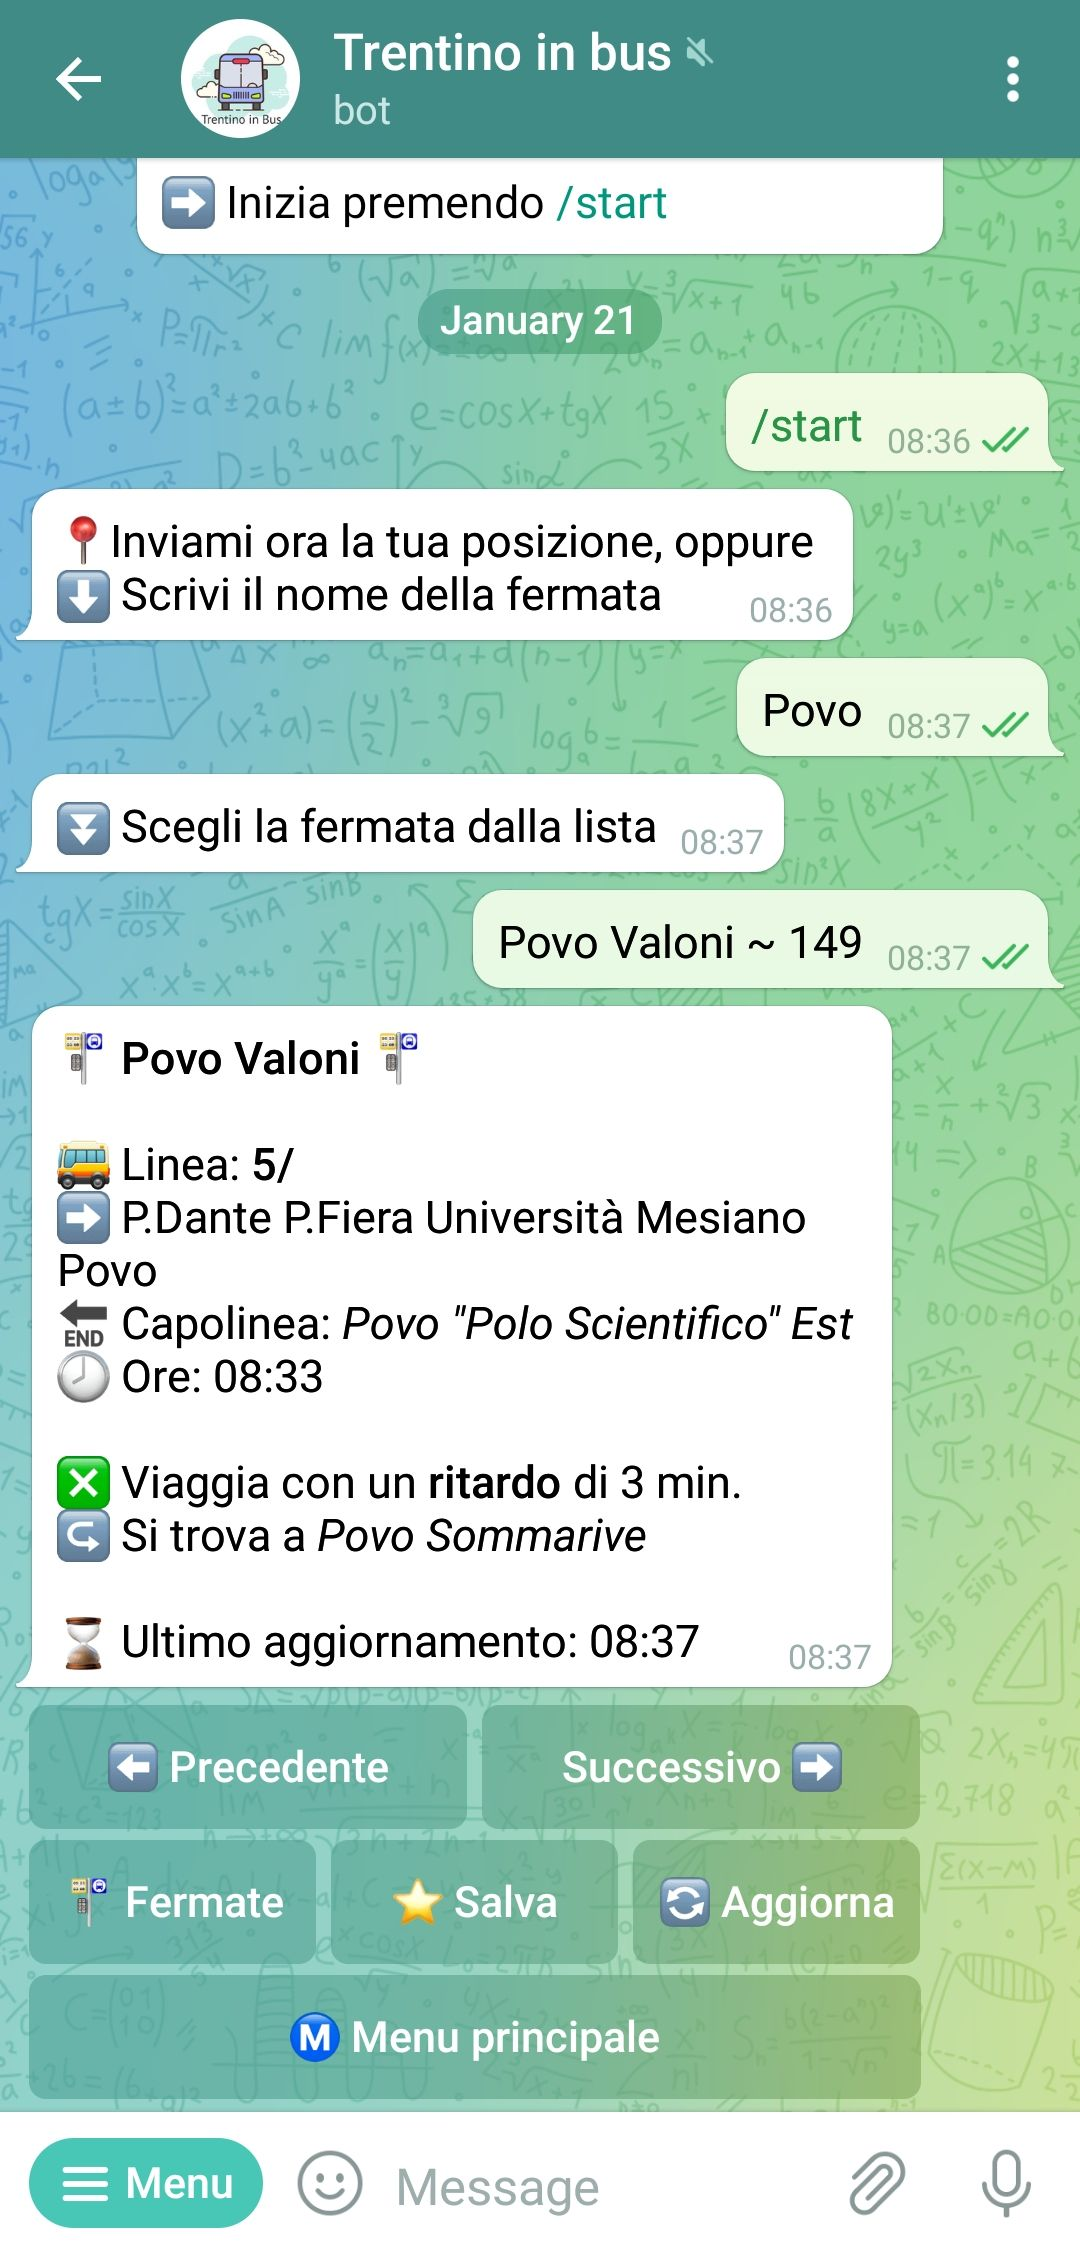
\includegraphics[width=\linewidth]{bot-orario-fermata.jpg}}
\caption{Orario fermata}
\label{fig:bot-orario-fermata}
\end{subfigure}\hfil 
\begin{subfigure}{0.20\textwidth}
\frame{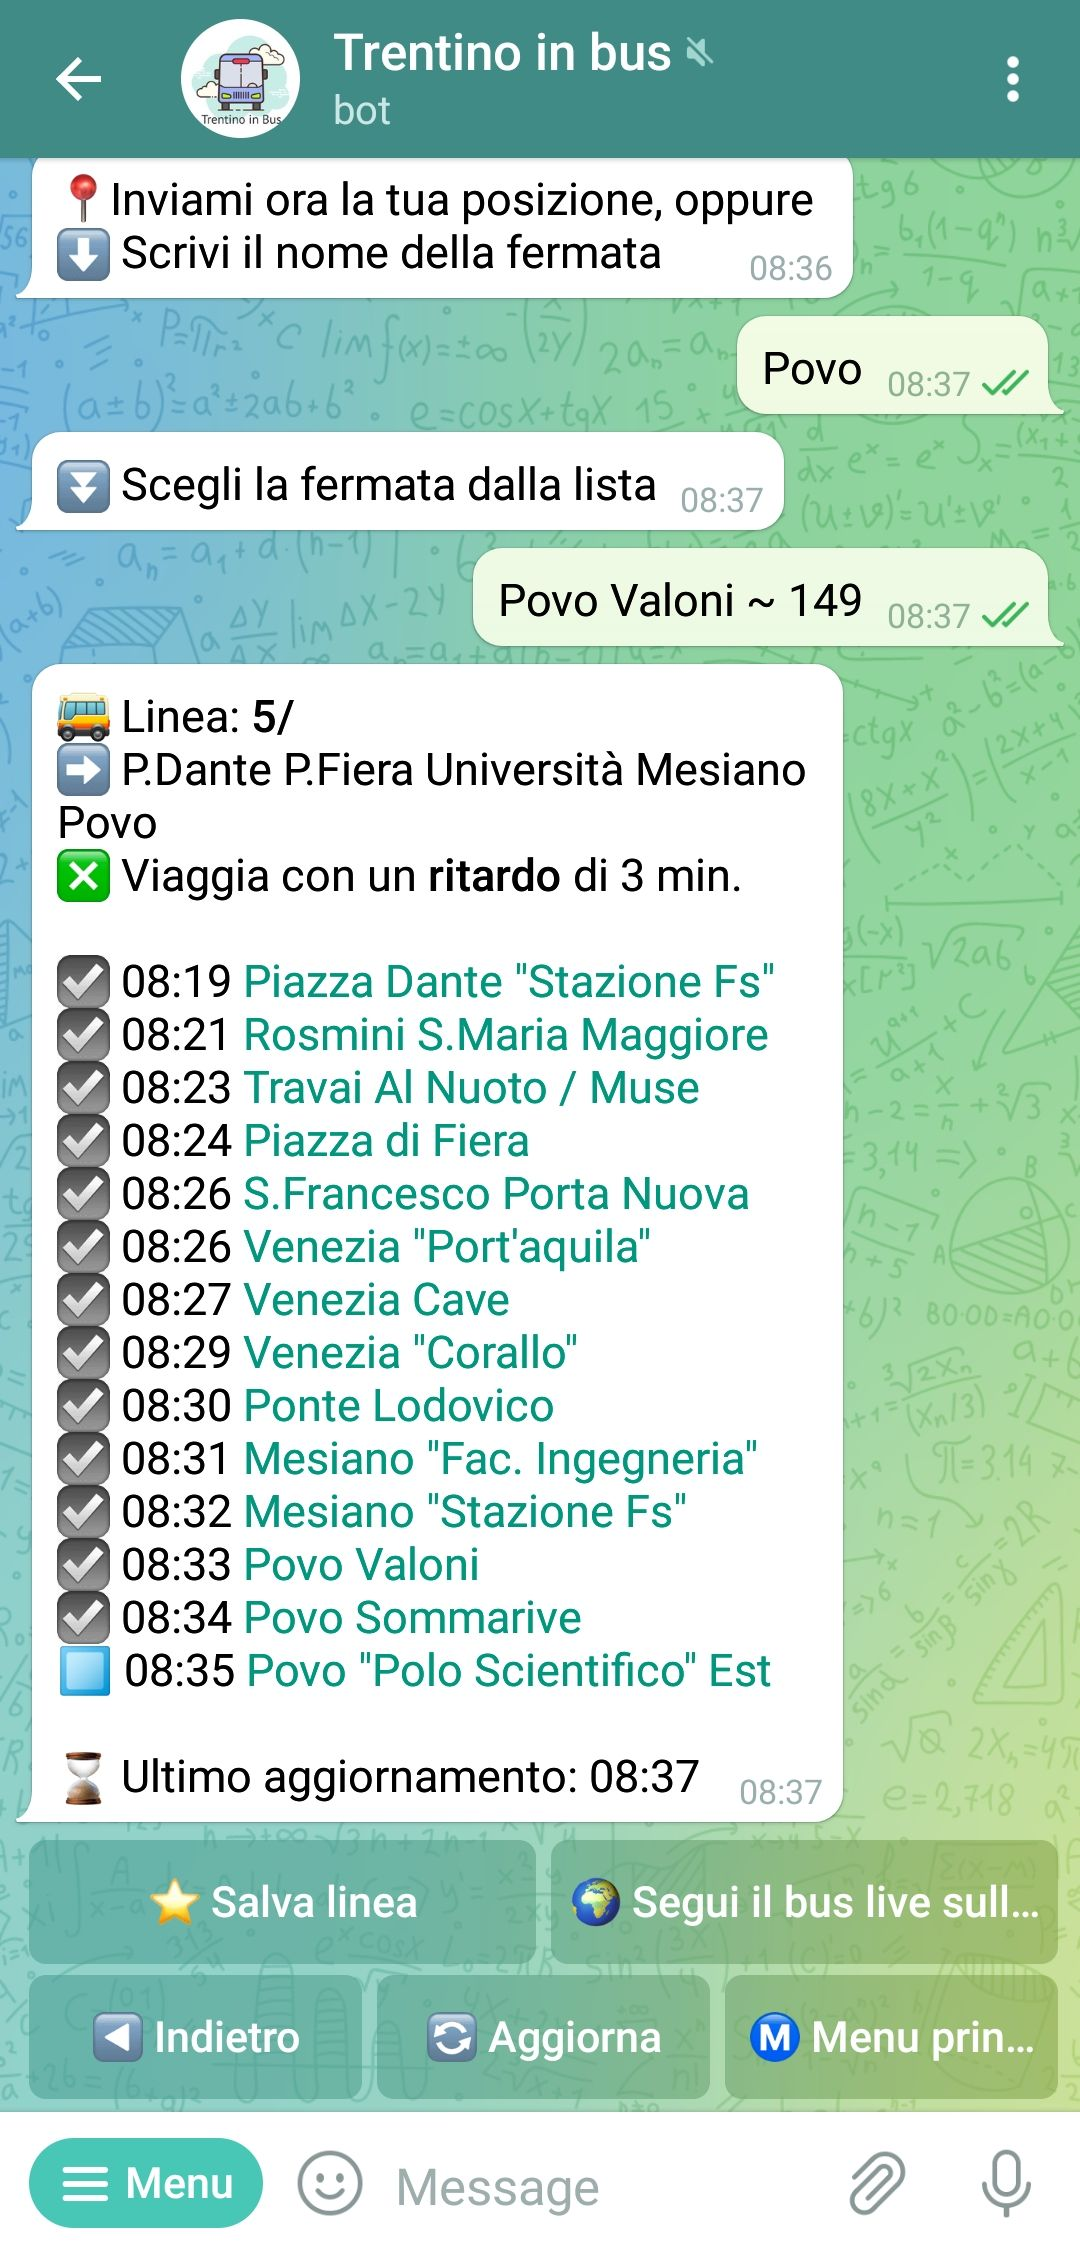
\includegraphics[width=\linewidth]{bot-orari-linea.jpg}}
\caption{Dettaglio linea}
\label{fig:bot-orari-linea}
\end{subfigure}
\caption{
\label{fig:autobus_interfaccia} Interfaccia funzionalità autobus}
\end{figure}

\begin{wrapfigure}{r}{0.33\textwidth}
\centering
\frame{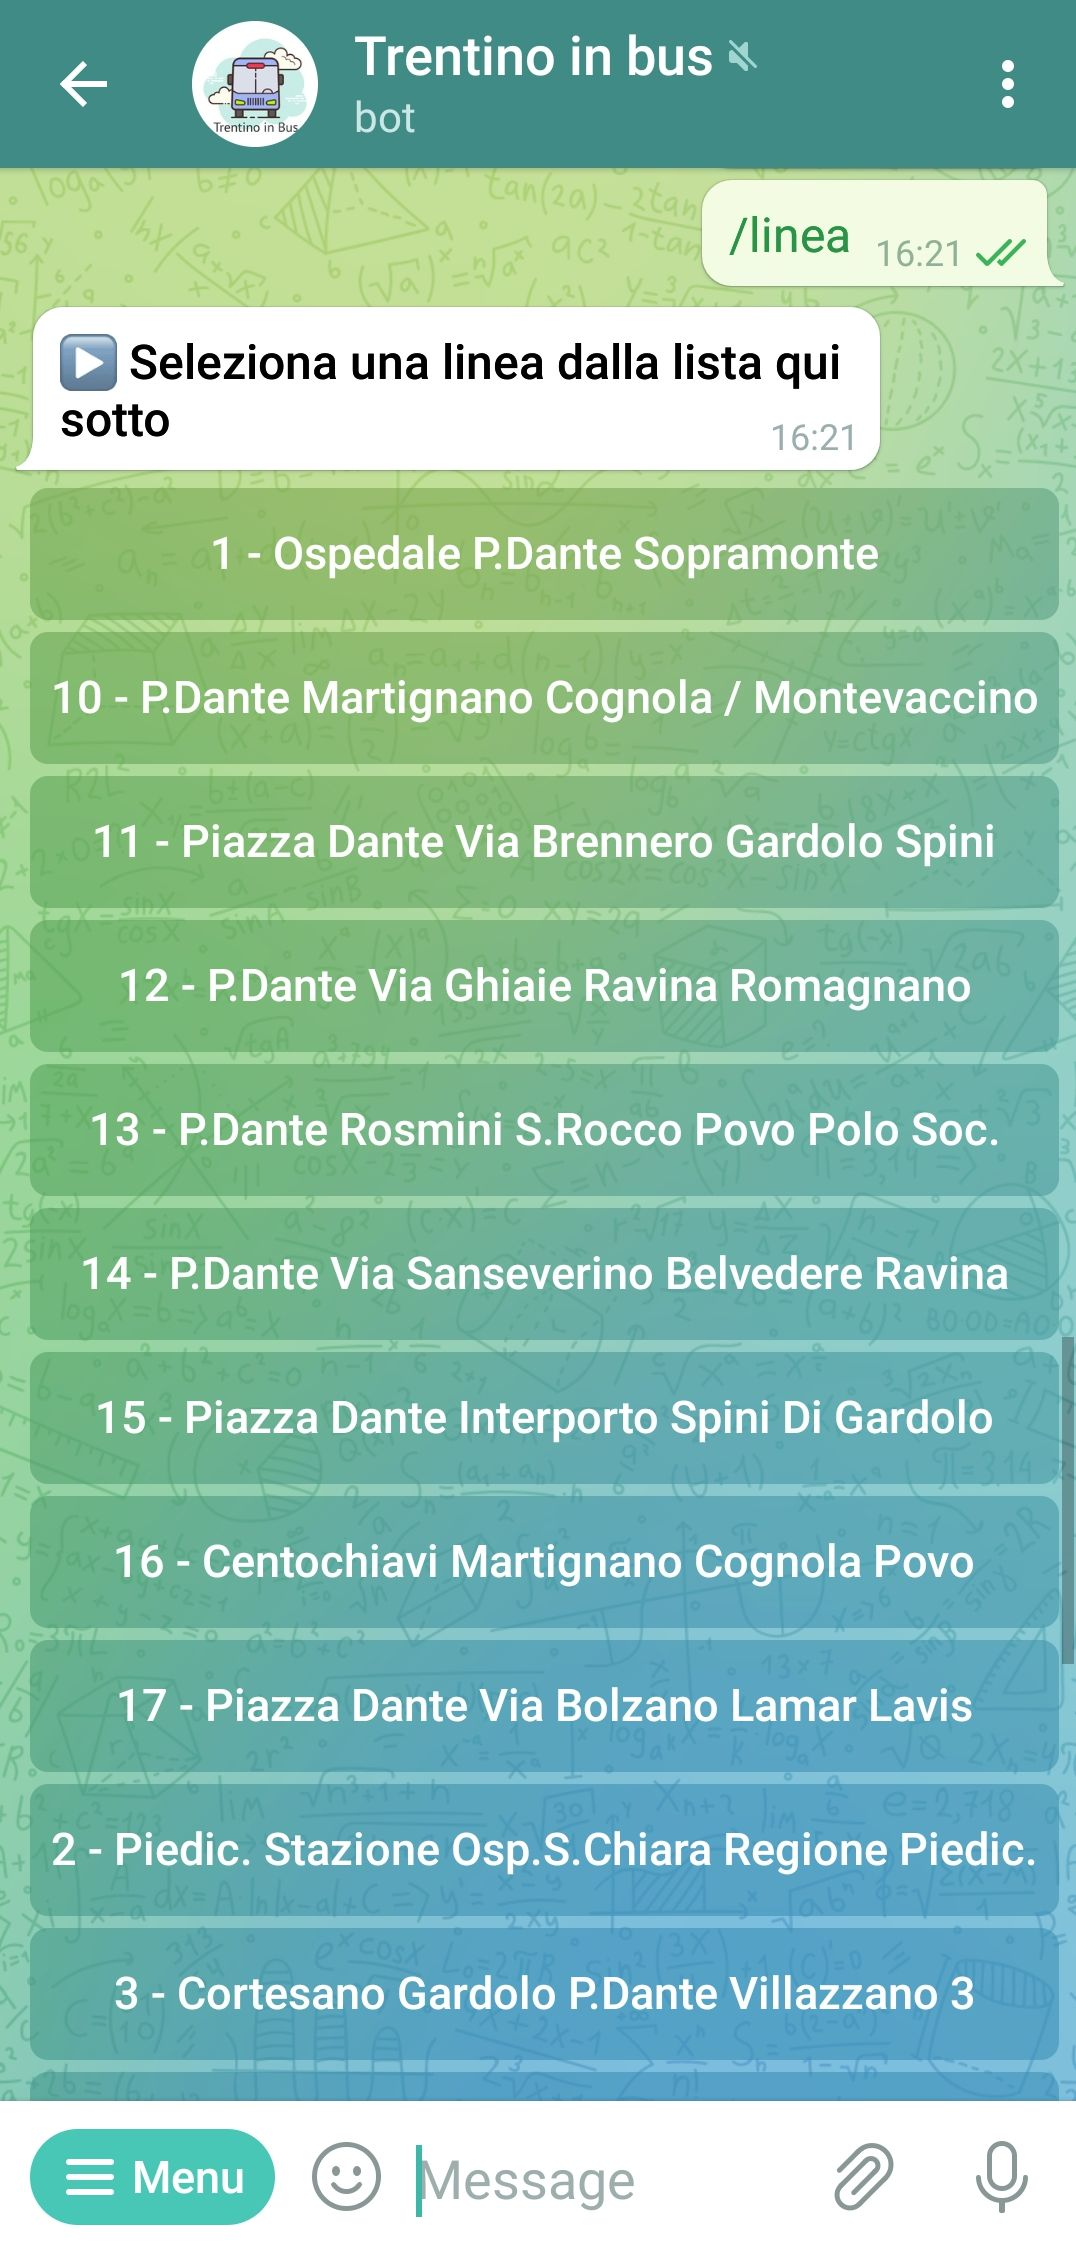
\includegraphics[scale=0.10]{bot-lista-linee.jpg}}
\caption{Lista linee}
\label{fig:bot-lista-linee}
\end{wrapfigure}

Nella figura \ref{fig:autobus_interfaccia} è descritto il funzionamento della funzionalità autobus, in particolare della ricerca degli orari di una fermata. All'utente, una volta premuto il pulsante \textit{Autobus} del menu principale, verrà chiesto se intende ricercare una fermata oppure una linea. Premendo sul pulsante \textit{fermata} dovrà poi scrivere il nome della fermata che sta ricercando oppure inviare la propria posizione, a questo punto, a seconda della scelta fatta in precedenza, il bot restituirà una lista di fermate con il nome simile o vicine alla posizione inviata. Dopo aver scelto la fermata di suo interesse, l'utente potrà visualizzare gli autobus in arrivo. Come si nota nella figura \ref{fig:autobus_interfaccia}\subref{fig:bot-orario-fermata} è possibile visualizzare il dettaglio di un solo autobus per volta e, utilizzando i pulsanti \textit{precedente} e \textit{successivo}, è possibile navigare tra gli arrivi. Nel messaggio di dettaglio è presente la linea, il capolinea, l'orario di partenza, l'eventuale ritardo e l'ultima posizione rilevata dell'autobus. Le informazioni in tempo reale si possono aggiornare utilizzando il bottone \textit{Aggiorna}, mentre il bottone \textit{Salva} permette all'utente di salvare la fermata nei propri preferiti. Con il bottone \textit{Fermate} si visualizzerà il messaggio visibile in figura \ref{fig:autobus_interfaccia}\subref{fig:bot-orari-linea}. Quest'ultimo fornisce il dettaglio dell'autobus mostrandone tutte le fermate con il relativo orario di arrivo. Anche qui si ha la possibilità di aggiungere la linea ai preferiti ed è inoltre possibile visualizzare la posizione del bus in tempo reale sulla mappa (funzionalità descritta nel paragrafo \ref{sec:altre_funzionalita}).

Nel caso in cui l'utente scegliesse di ricercare una linea invece che una fermata, il bot proporrà una lista di linee (figura \ref{fig:bot-lista-linee}). L'utente, dopo averne selezionata una, si troverà di fronte un messaggio simile a quello presentato in figura \ref{fig:autobus_interfaccia}\subref{fig:bot-orari-linea} con l'aggiunta, anche in questo caso, dei bottoni \textit{precedente} e \textit{successivo} per navigare tra gli orari.

\subsection{Funzionalità ferrovie}

\begin{wrapfigure}{r}{0.55\textwidth}
    \centering 
\begin{subfigure}{0.23\textwidth}
\centering
\frame{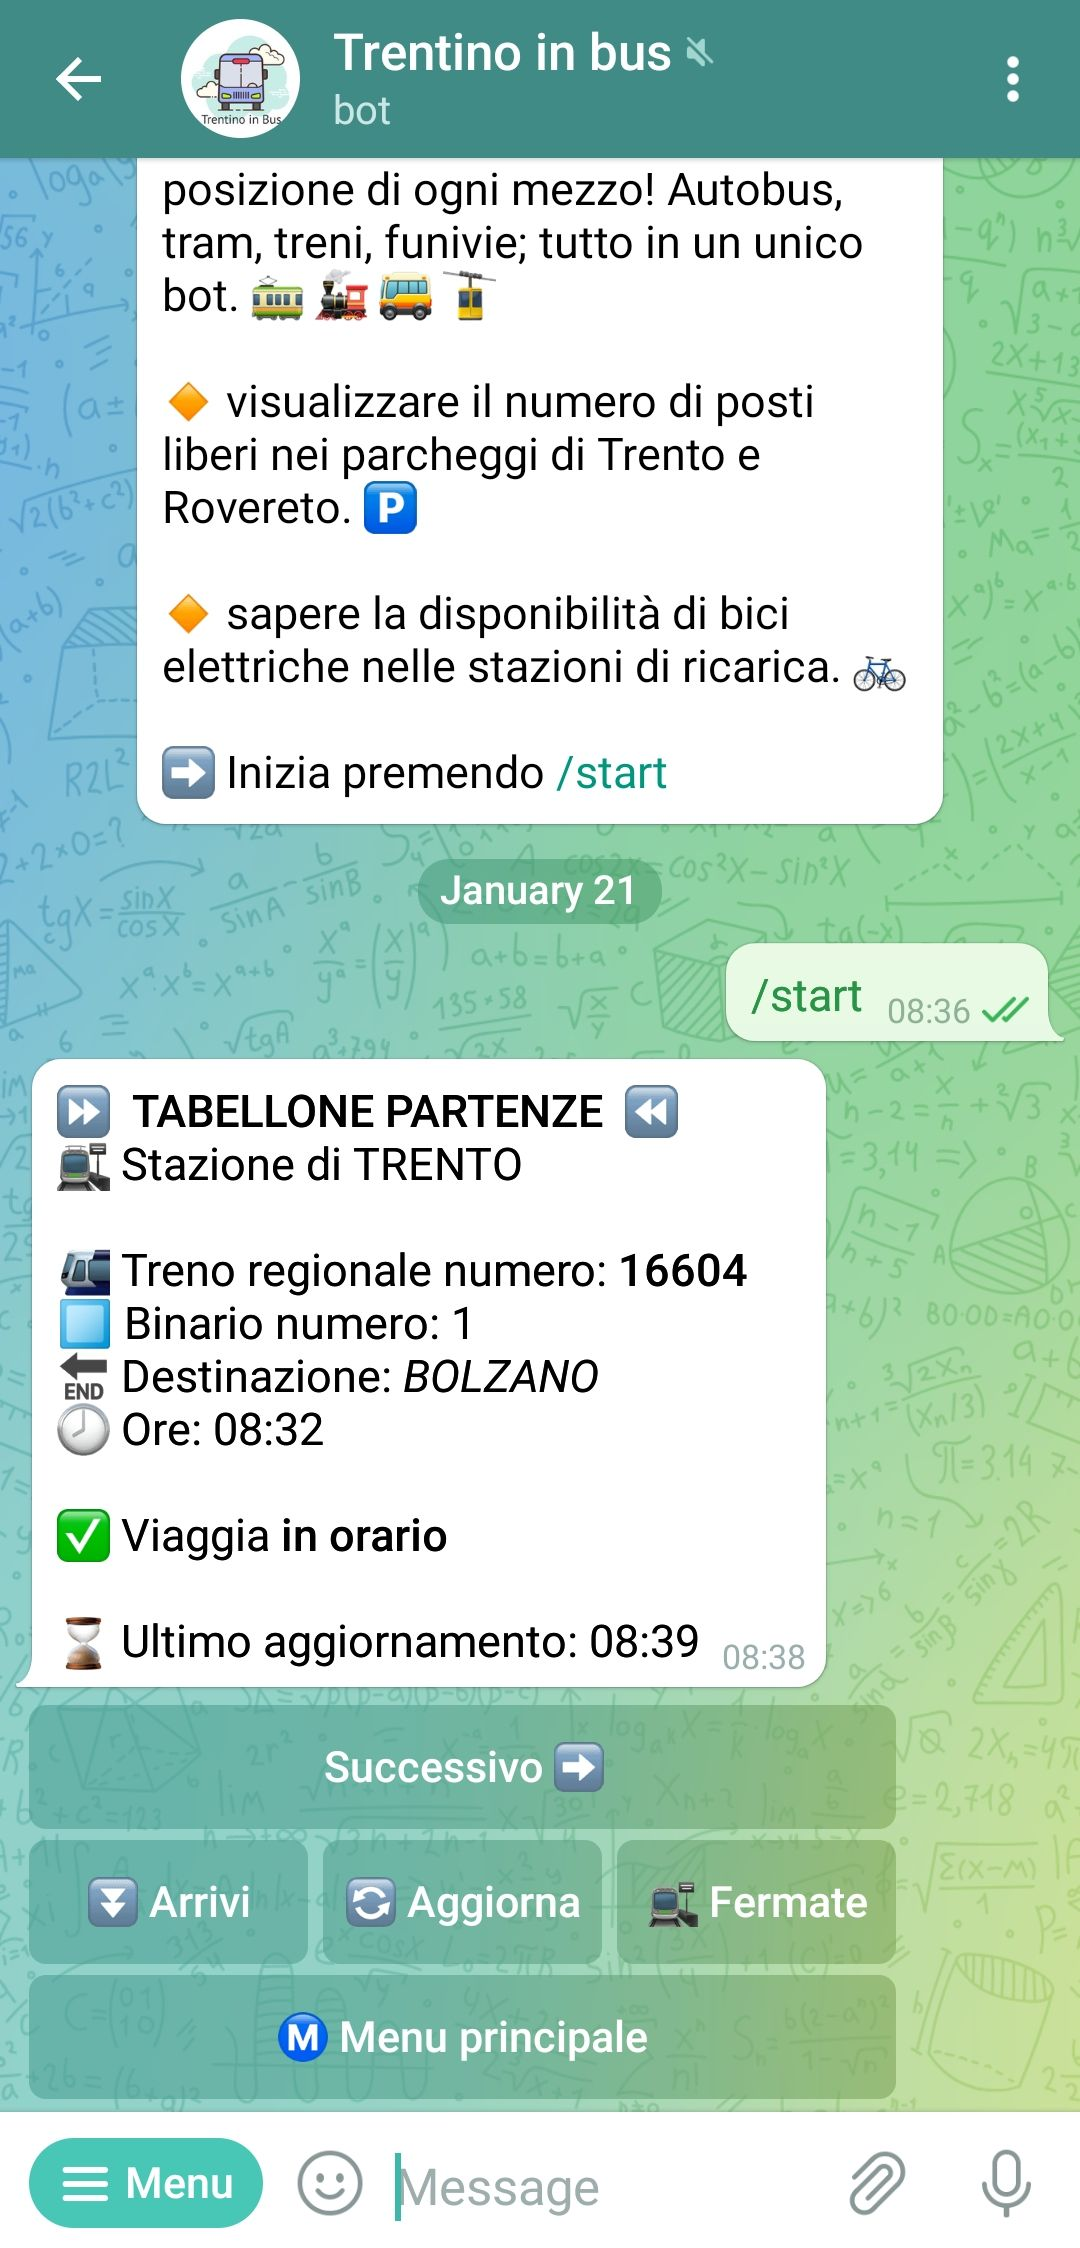
\includegraphics[scale=0.1]{bot-partenze-treno.jpg}}
\caption{Partenze stazione}
\label{fig:bot-partenze-treno}
\end{subfigure}\hfil
\begin{subfigure}{0.23\textwidth}
\centering
\frame{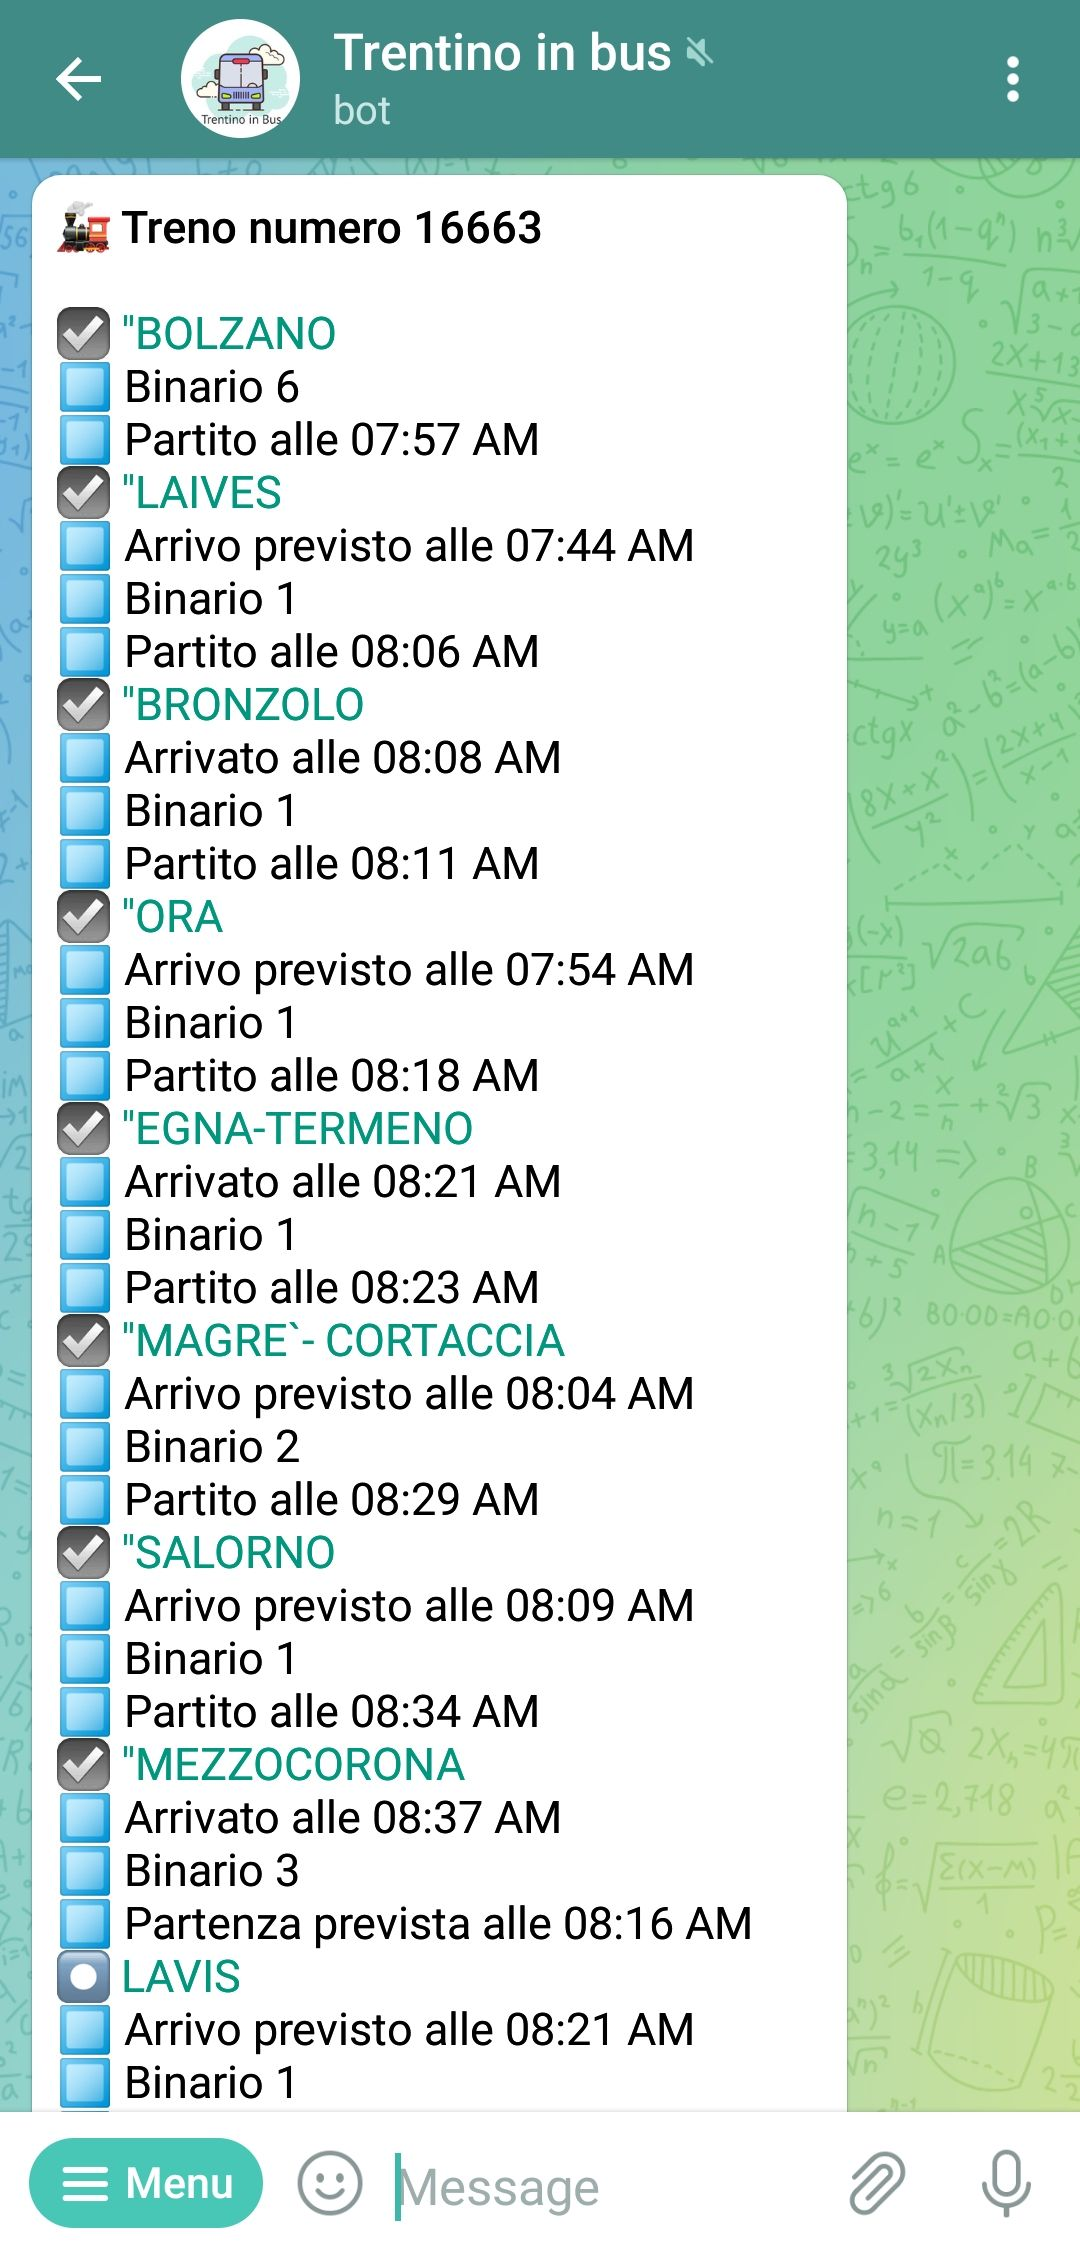
\includegraphics[scale=0.1]{bot-fermate-treno.jpg}}
\caption{Orari fermate}
\label{fig:bot-fermate-treno}
\end{subfigure}
\caption{
\label{fig:treni_interfaccia}Interfaccia funzionalità treni}
\end{wrapfigure}

L'interfaccia della funzionalità ferrovie, esposta in figura \ref{fig:treni_interfaccia}, è molto simile alla funzionalità autobus, ma presenta alcune differenze. Una volta premuto sul bottone \textit{Ferrovie} del menu principale, l'utente dovrà scegliere la ferrovia da visualizzare tra Valsugana, Brennero e Trento-Mezzana. 

Nel caso delle ferrovie gestite da Trenitalia (Valsugana e Brennero) l'utente dovrà scegliere la fermata di suo interesse da una lista e successivamente potrà visualizzarne le partenze e gli arrivi con un messaggio somigliante a quello descritto in precedenza per gli autobus. Anche in questo caso premendo il pulsante \textit{Fermate} l'utente visualizzerà un messaggio con il dettaglio delle fermate del treno, con il relativo binario e gli orari di arrivo e di partenza. Come per gli autobus, anche per i treni, si hanno informazioni in tempo reale sull'ultima posizione rilevata e sull'eventuale ritardo.

L'interfaccia dei messaggi per la ferrovia Trento-Mezzana, a differenza delle ferrovie di Trenitalia, non presenta il binario e l'orario di arrivo coincide sempre con quello di partenza.

\pagebreak

\subsection{Altre funzionalità}
\label{sec:altre_funzionalita}

Il bot presenta altre funzionalità minori, in particolare:

\begin{itemize}
\item la sezione preferiti, dove possiamo trovare le linee e/o fermate salvate in precedenza al fine di visualizzarne gli orari più velocemente (figure \ref{fig:varie_funzionalita}\subref{fig:bot-preferiti}, \ref{fig:varie_funzionalita}\subref{fig:bot-fermate-preferite});

\item la visualizzazione della disponibilità di biciclette nelle stazioni di ricarica, gli slot totali e quelli liberi (figura \ref{fig:varie_funzionalita}\subref{fig:bot-stazioni-bici});

\item i parcheggi disponibili nelle città di Trento e Rovereto, per ognuno di questi, se monitorati, è possibile vedere i posti liberi e quelli totali; 

\item la possibilità di visualizzare la posizione di un autobus in tempo reale sulla mappa. Per una limitazione delle API non è possibile avere le informazioni GPS, ma solo quelle dell'ultima fermata effettuata. (figura \ref{fig:varie_funzionalita}\subref{fig:bot-posizione-autobus}) 
\end{itemize}

\begin{figure}[htb]
    \centering 
\begin{subfigure}{0.20\textwidth}
\frame{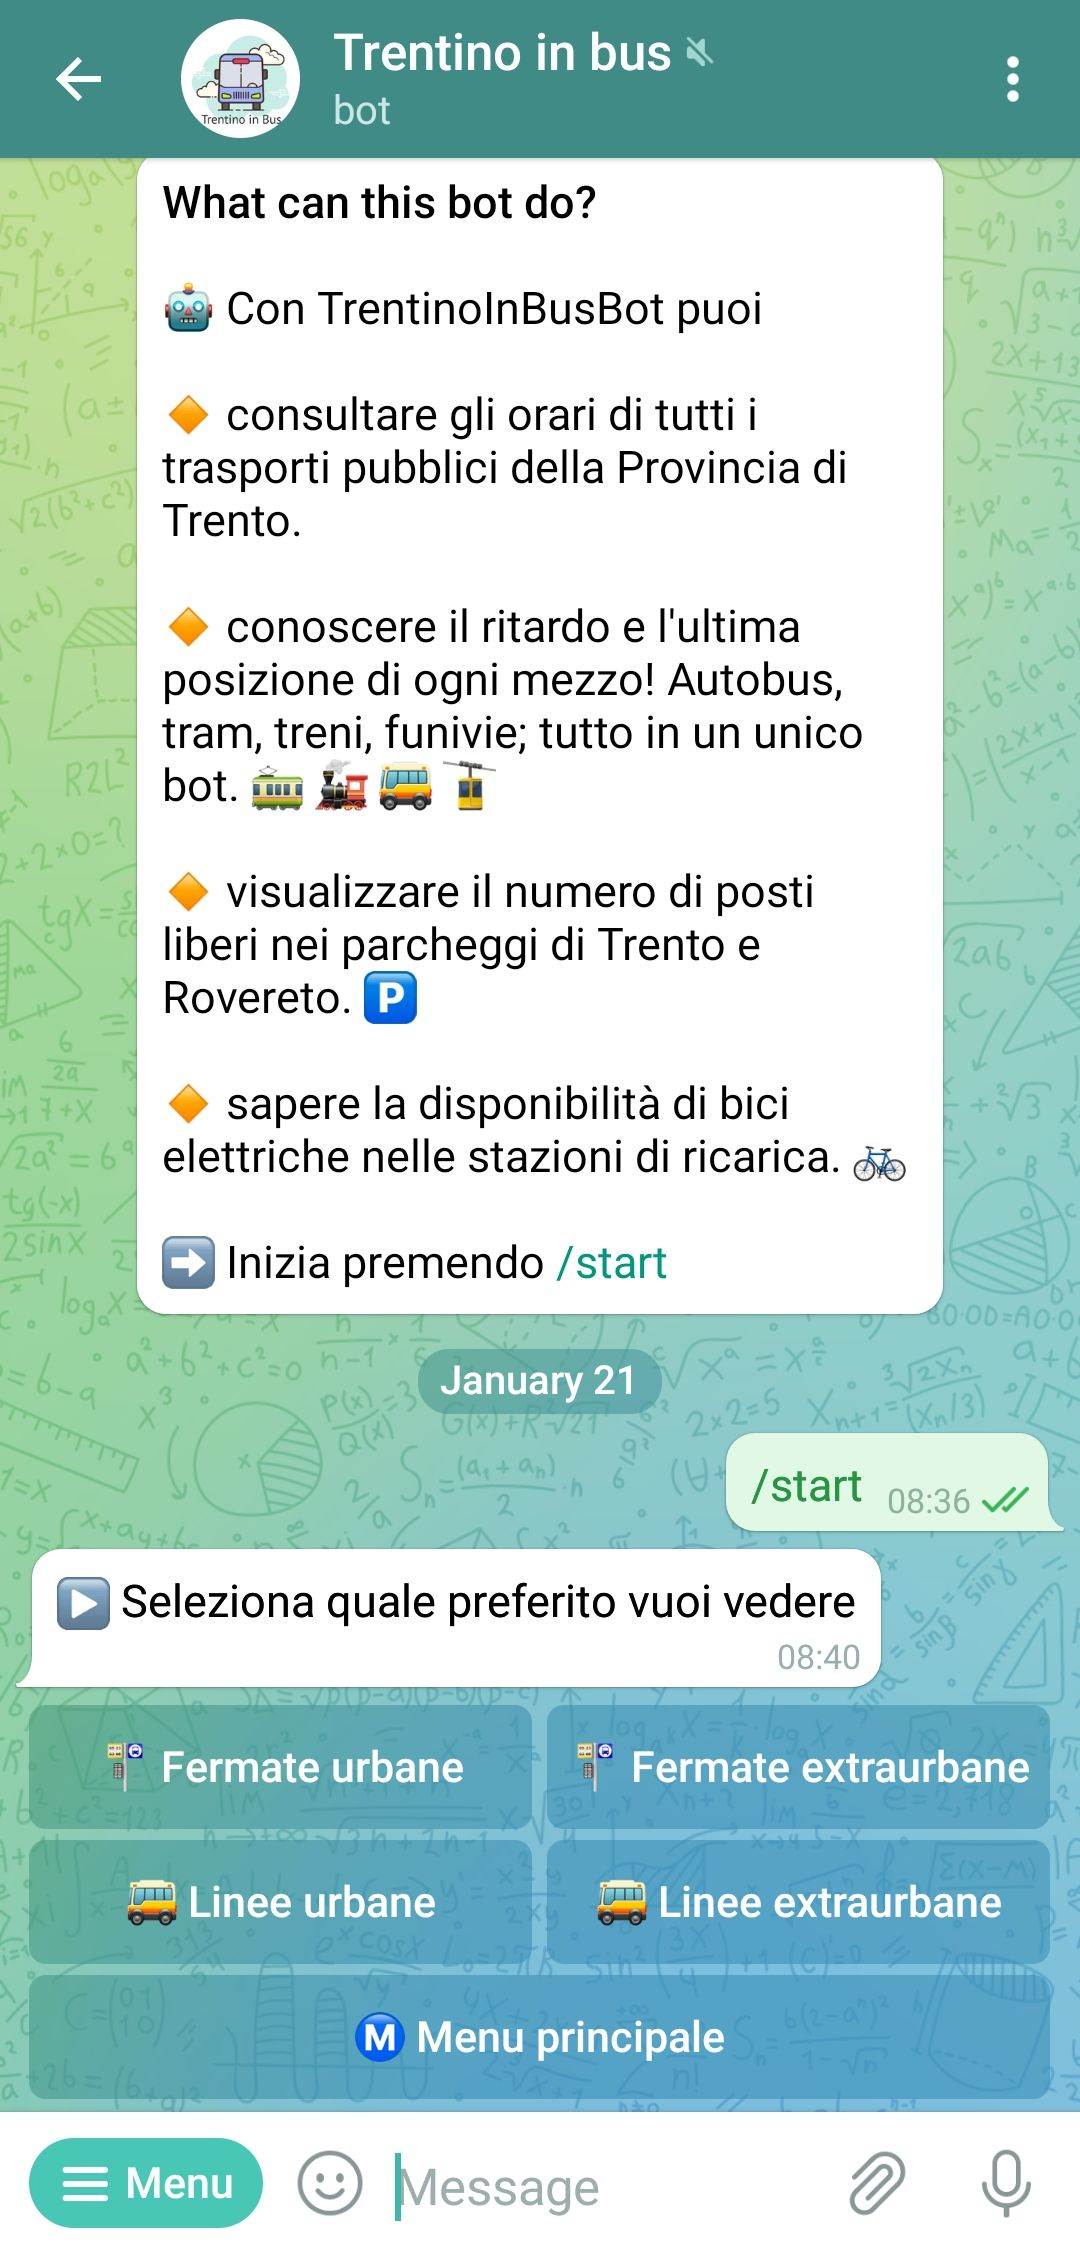
\includegraphics[width=\linewidth]{bot-preferiti.jpg}}
\caption{Preferiti}
\label{fig:bot-preferiti}
\end{subfigure}\hfil
\begin{subfigure}{0.20\textwidth}
\frame{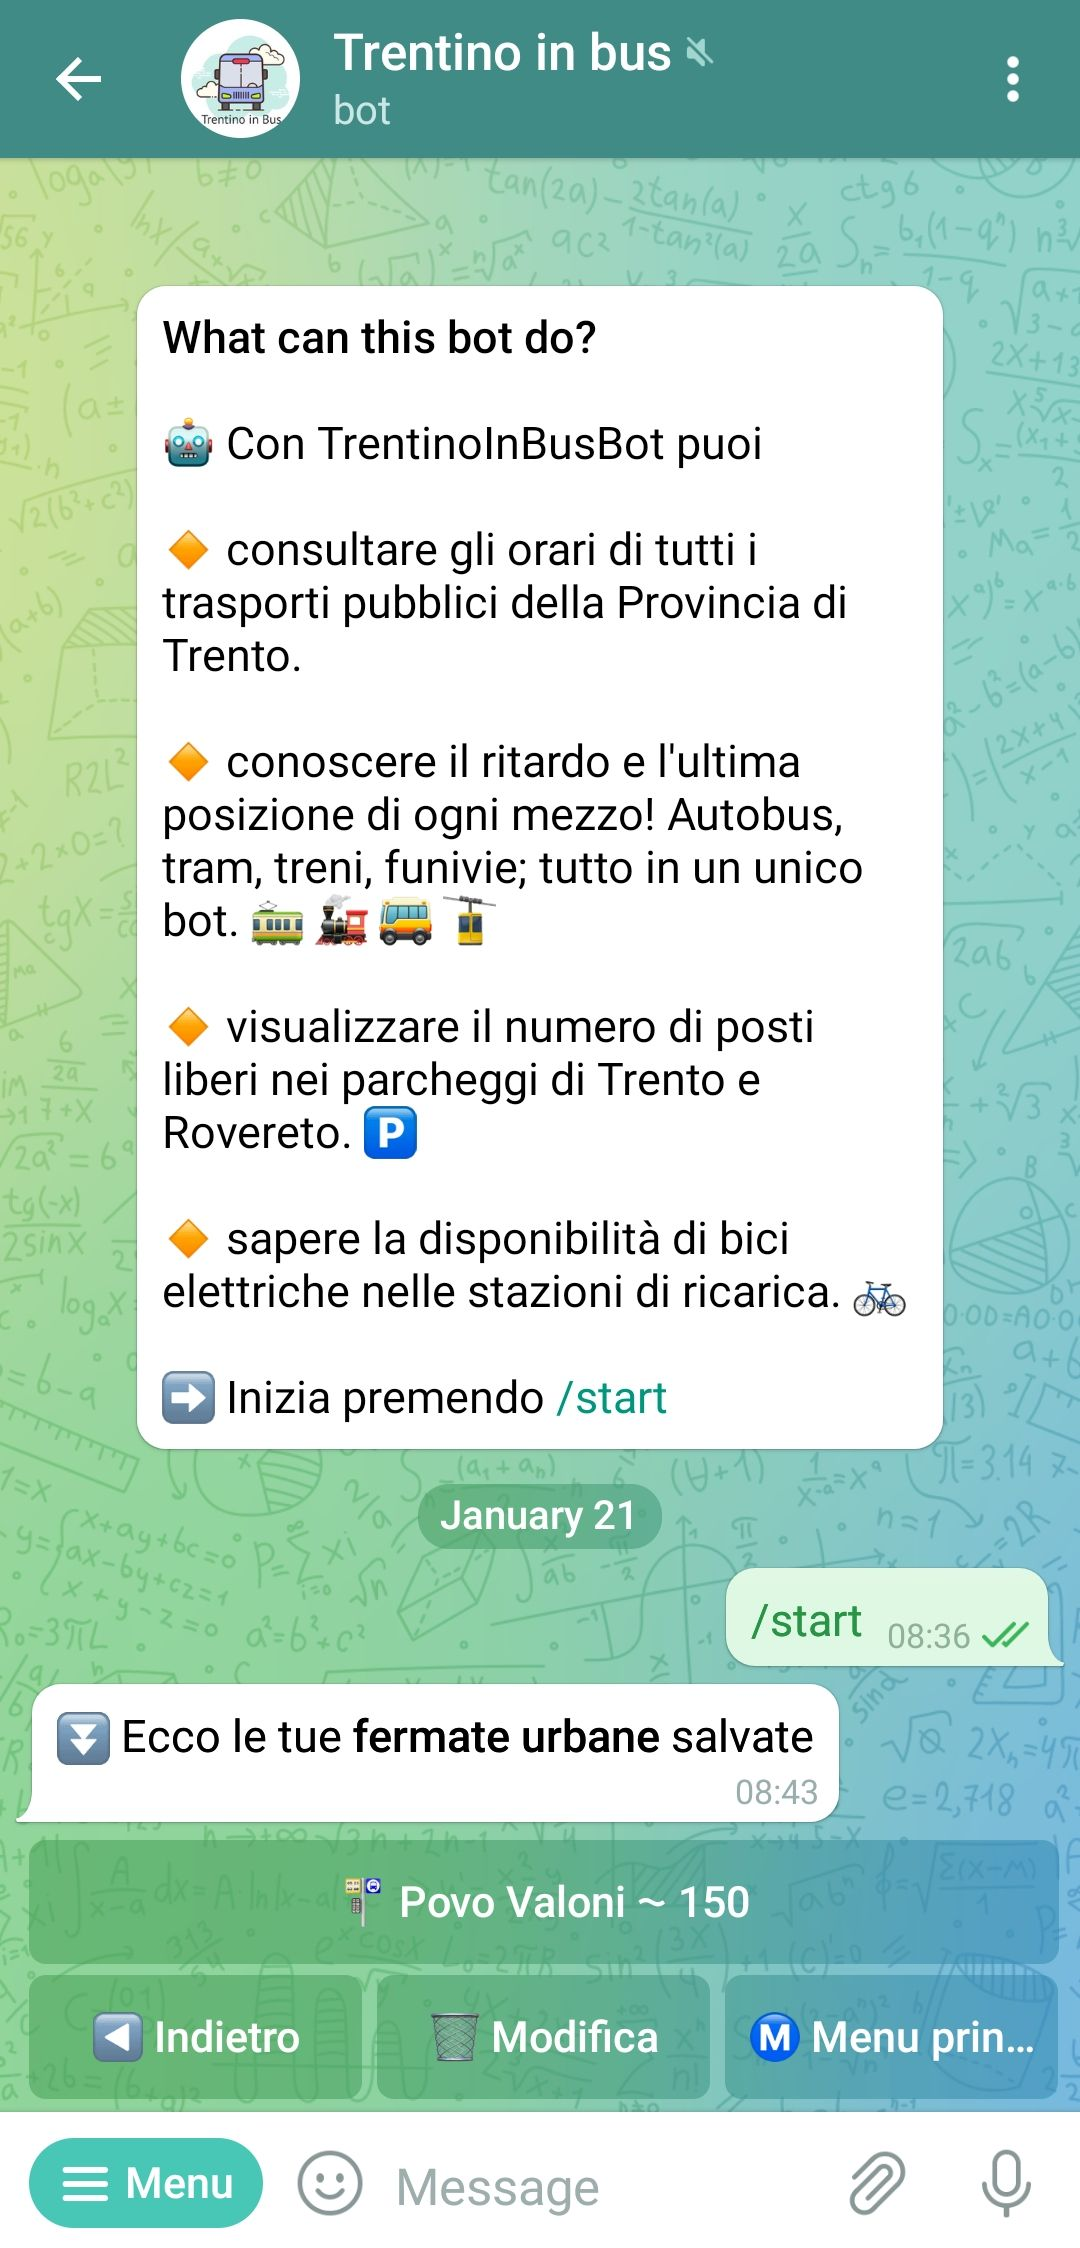
\includegraphics[width=\linewidth]{bot-fermate-preferite.jpg}}
\caption{Fermate preferite}
\label{fig:bot-fermate-preferite}
\end{subfigure}\hfil 
\begin{subfigure}{0.20\textwidth}
\frame{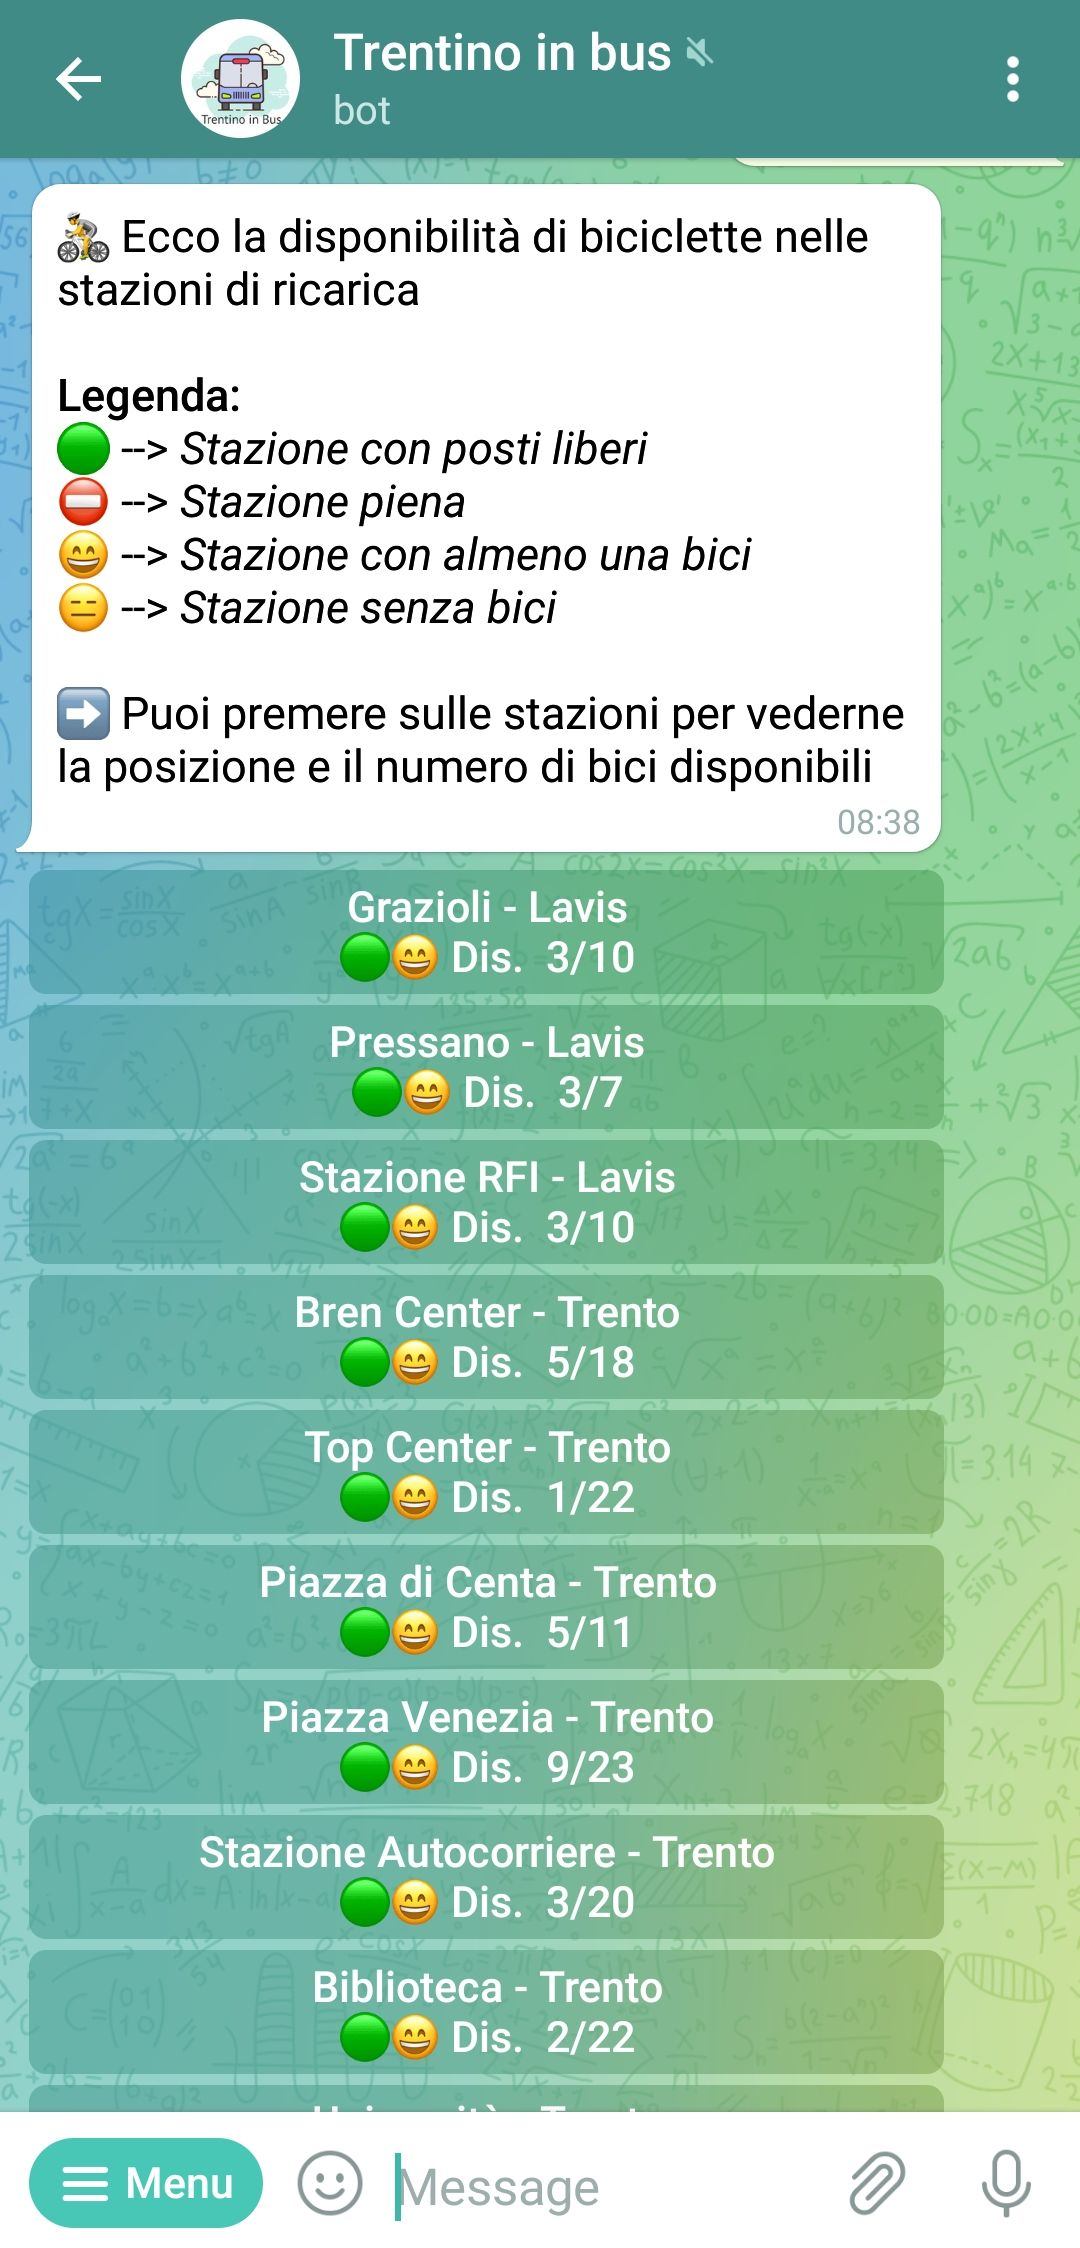
\includegraphics[width=\linewidth]{bot-stazioni-bici.jpg}}
\caption{Stazioni bici}
\label{fig:bot-stazioni-bici}
\end{subfigure}\hfil 
\begin{subfigure}{0.20\textwidth}
\frame{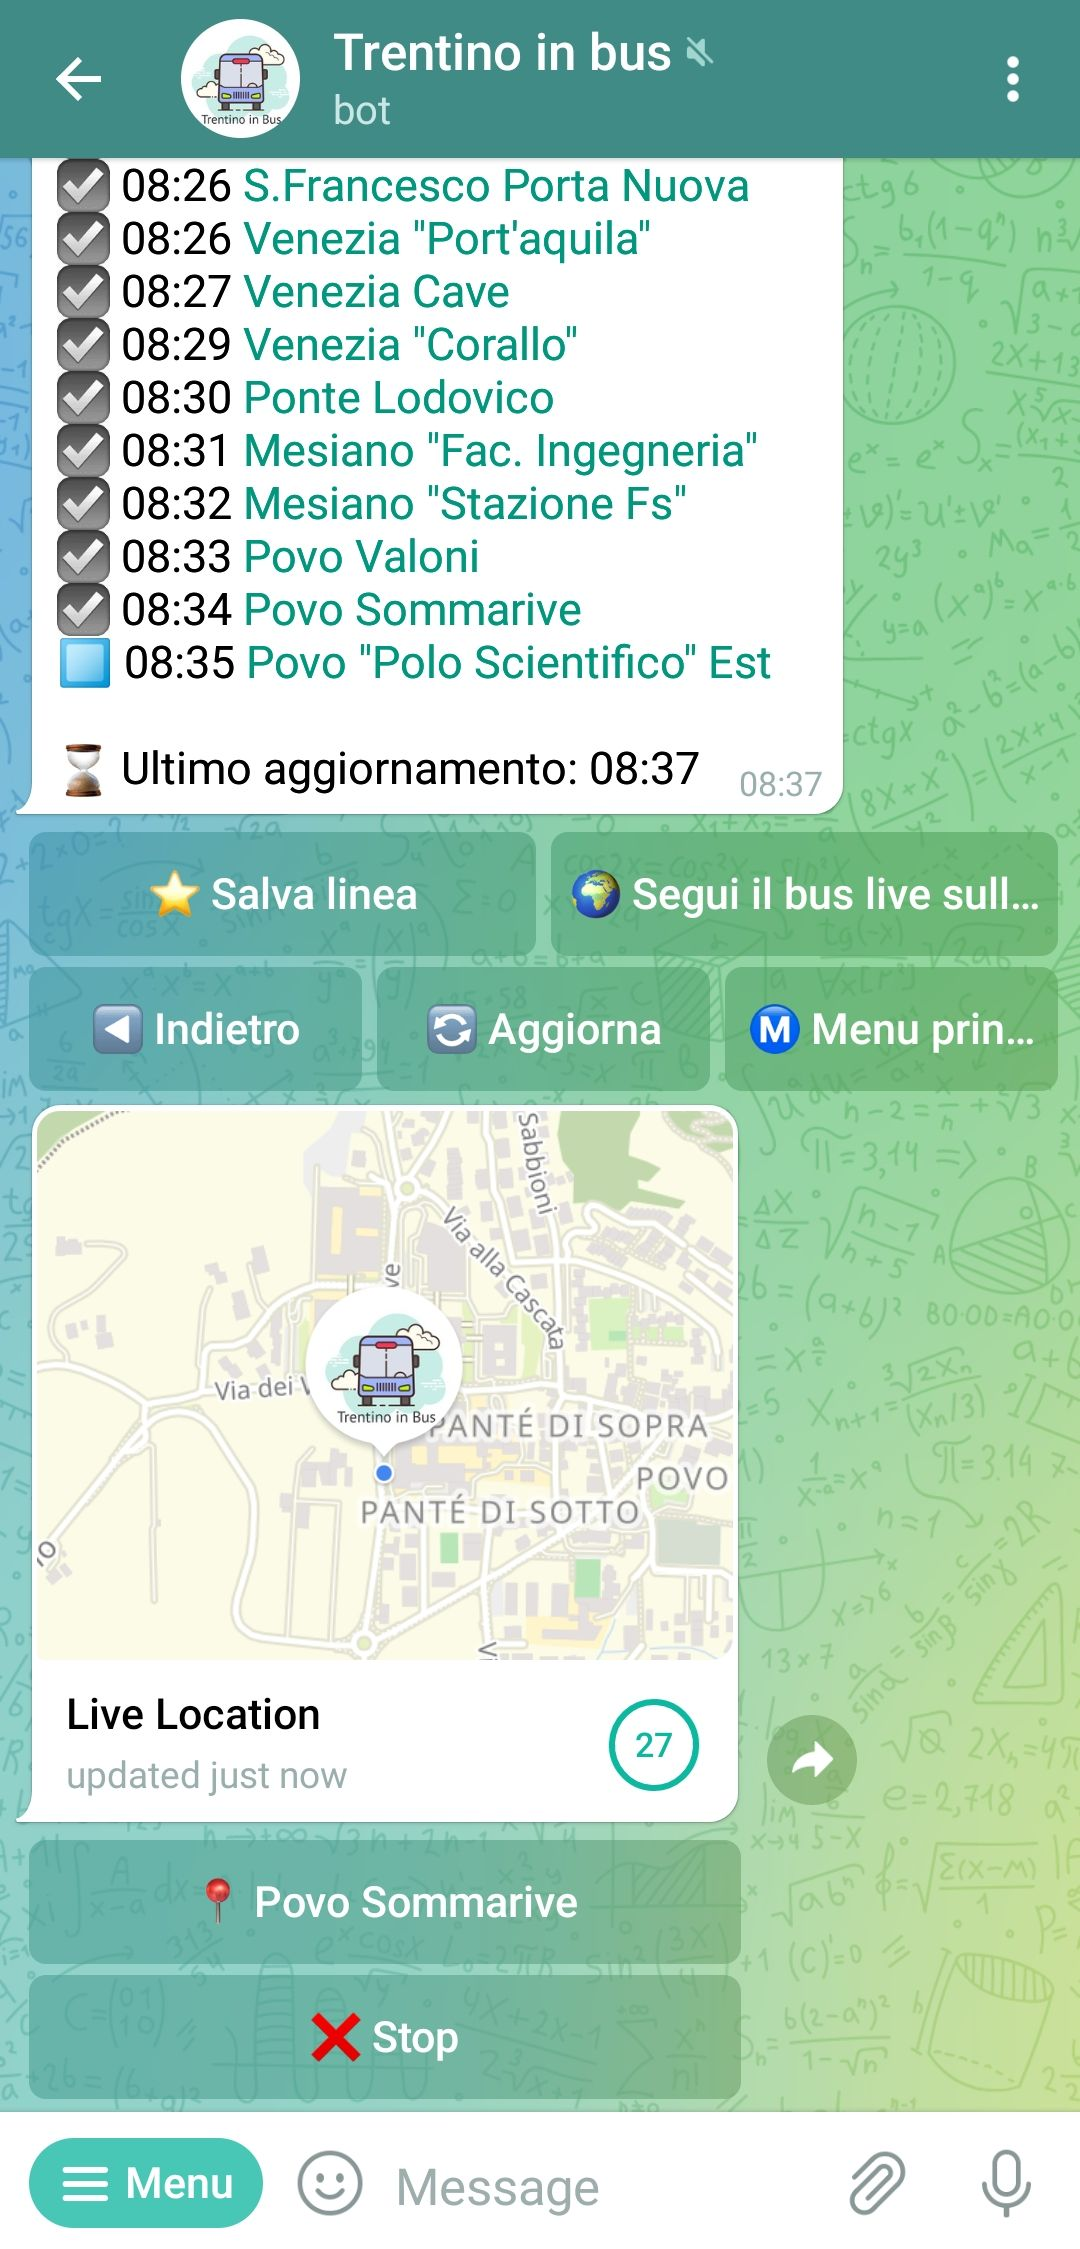
\includegraphics[width=\linewidth]{bot-posizione-autobus.jpg}}
\caption{Posizione autobus}
\label{fig:bot-posizione-autobus}
\end{subfigure}
\caption{
\label{fig:varie_funzionalita}Altre funzionalità}
\end{figure}


\subsection{Canale notizie}

\begin{wrapfigure}{r}{0.38\textwidth}
\centering
\frame{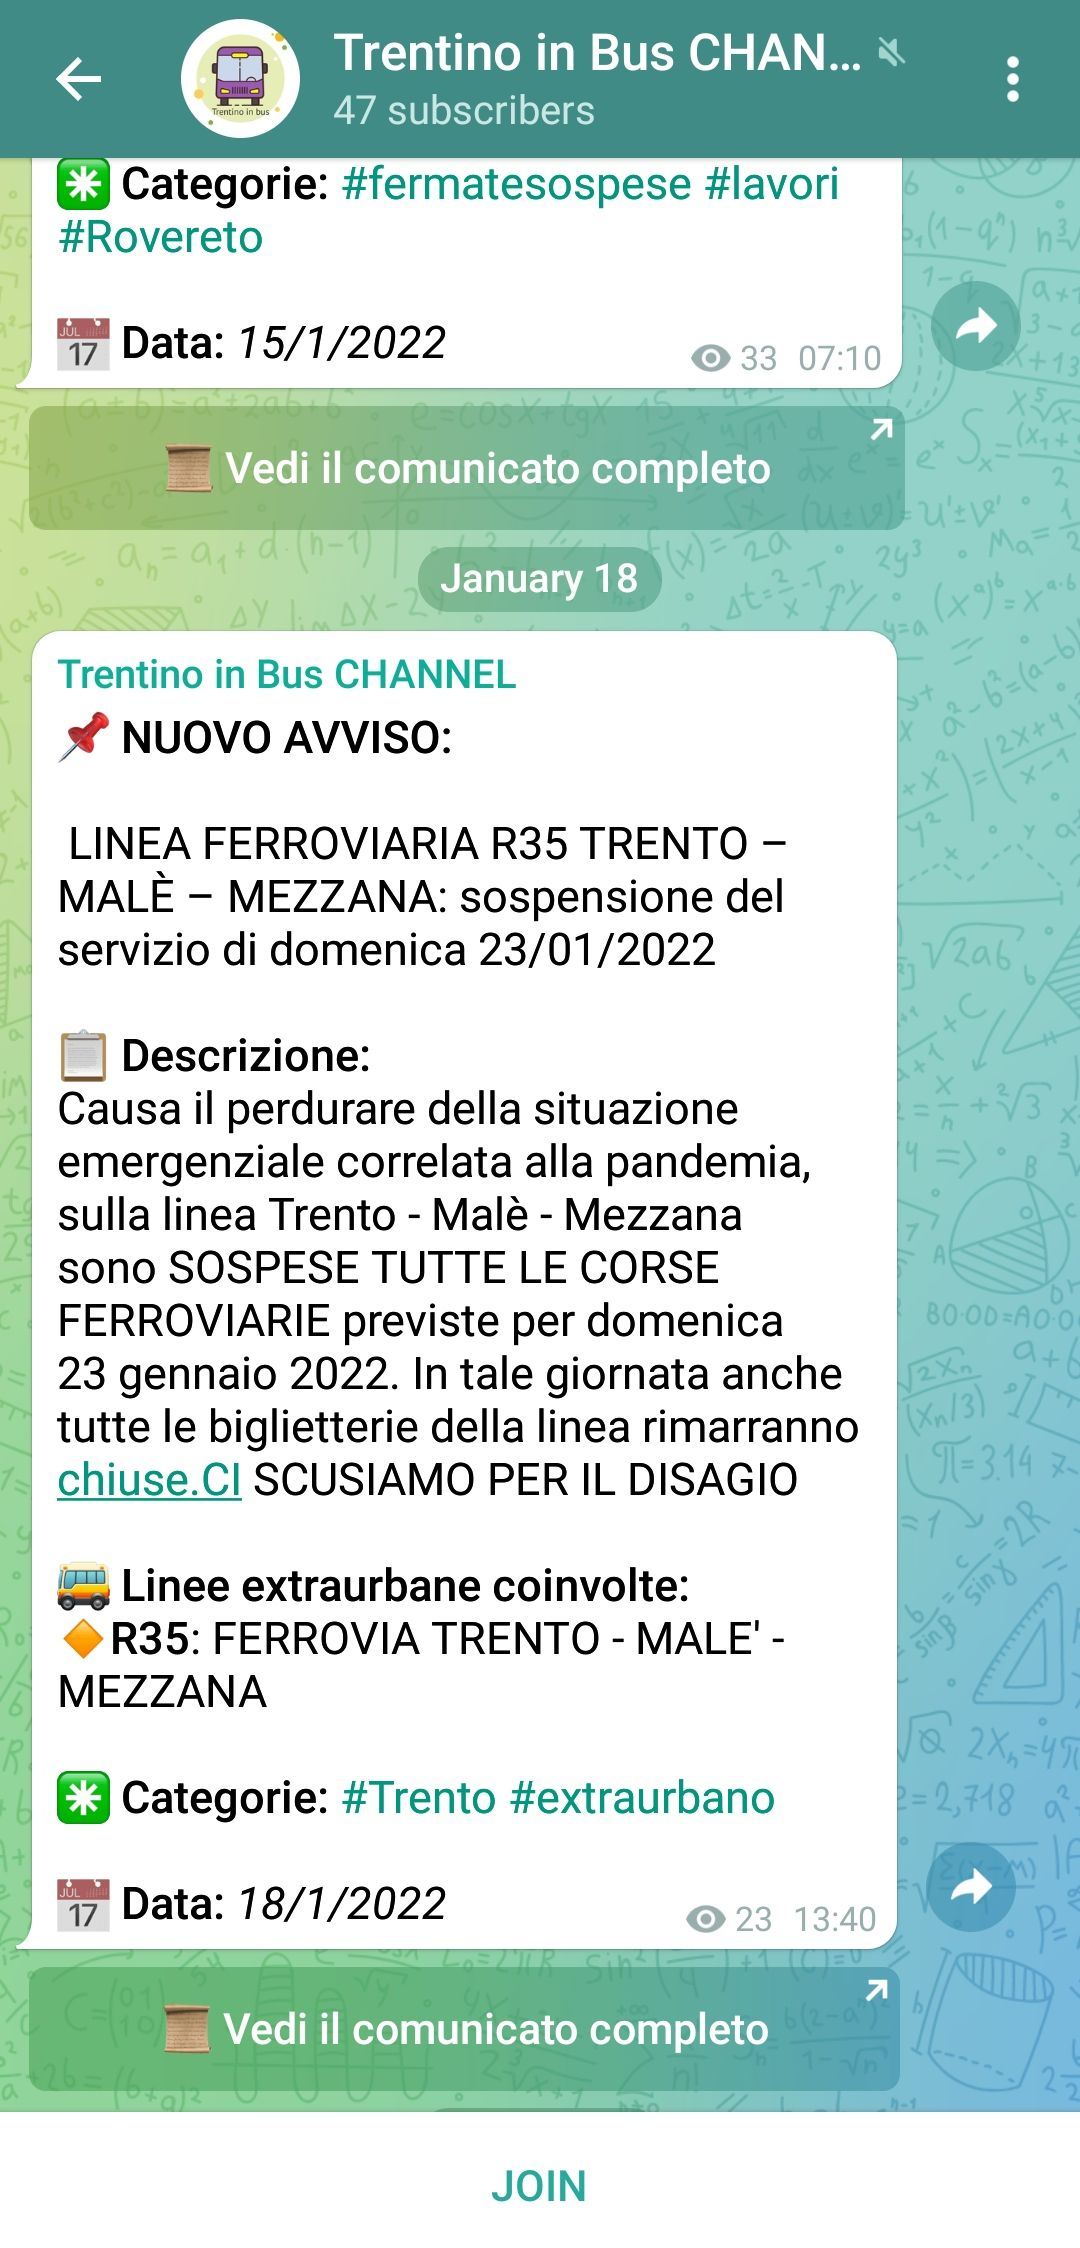
\includegraphics[scale=0.085]{bot-canale-notizie.jpg}}
\caption{Canale notizie}
\label{fig:bot-canale-notizie}
\end{wrapfigure}

Al bot principale \textit{@TrentinoInBusBot} è associato anche un canale Telegram, \textit{@TrentinoInBusChannel}, che si occupa di inviare agli iscritti aggiornamenti in tempo reale sui trasporti della Provincia di Trento. 

Questo canale è moderato automaticamente dal bot che invia al suo interno messaggi riguardanti scioperi, fermate sospese, variazioni di percorso, cambiamenti di orario, corse sospese, nuove corse e molto altro. I messaggi contengono un breve riepilogo della notizia e l'indicazione delle linee e fermate coinvolte. Anche in questo canale, come nel bot principale, i messaggi sono arricchiti dall'utilizzo di \textit{emoji} per renderli più chiari e accattivanti.

Le notizie di questo canale sono filtrabili attraverso dei tag per categoria in modo da essere facilmente ricercabili dagli utenti. Ad ogni messaggio è allegato un pulsante attraverso il quale è possibile scaricare il PDF del comunicato ufficiale di Trentino Trasporti.